% !TEX root=frame_thesis.tex
\chapter{Development of an Agent-Based Model for Easter Island of Human Resource Interaction}\label{chapter:Methods}
\FloatBarrier
\section{Model Overview}
%Topic: General overview of ABM
%Main Idea: Human agents interact with local Environment
\paragraph{General Description.}
I present an Agent-Based Model (ABM) that simulates the spatial and temporal history of household agents on Easter Island and their interactions with the natural environment. 
The environment is encoded on a 2D discretised map with heterogeneous geographic and biological features.
Agents rely both on a limited, non-(or slowly) renewable resource, the palm trees, and a limited resource, farming conducted on arable land (in particular, sweet potatoes).
Agents obtain these resources by cutting trees and farming viable sites in their near surroundings and, thereby, changing their local environment.
Some agents living close to Anakena Beach replace farming activity with fishing and, hence, do not need to occupy farming sites.
The household's population growth or decline, consequently, depends on the success of this resource acquisition. 
Furthermore, resource availability and other geographic indicators determine the moving behaviour of the agents.
The interaction with the natural environment, thus, constrains the moving patterns as well as the dynamics of the population size of the Easter Island society.

%Topic: Time and Update Order
\paragraph{Handling of Events and Time.}
The model assumes yearly updates of the characteristic variables of each household agent and the environment throughout the simulated time period.
The simulation starts with the arrival of the first settlers at Anakena Beach in
\begin{equation}
t_\text{arrival} = 800\, {\rm A.D.}\ ,
\end{equation}
following \citet{Bahn2017}\footnote{Other arrival dates are discussed in Section \ref{sec:PopGrowth}.}.
The initial population is assumed to be $\mathbf{pop}_{\rm arrival} = 40$ individuals (as in \citen{Brander1998}, and similar to \citen{Brandt2015}) spread on $2$ households, that both settle close to Anakena Beach (in the North, see Figure \ref{fig:Karte}).
After each time step, $\Delta t=1\,{\rm yr}$, all agents are updated and interact with their local environment sequentially in a randomised order. 
New household agents can appear throughout the simulation following reproduction and splitting of existing agents. 
Following the alteration of the environment by all agents, the environment's state variables are updated (e.g.\ potential regeneration, or soil degradation) once per year (`environmental update').
The simulation ends in $1900\, {\rm A.D.}$ with the arrival of frequent European voyagers, slave trade and European diseases marking the end of the isolated status of the historic Easter Island society .%, since this presumably had a large impact on the society, e.g.\ through the introduction of diseases wiping out a large fraction of the Easter Island population in the 19th century.% \todo{cite Bahn2017}.
%\begin{algorithm}
%	\caption{General Structure}
%	\STATE $t=t_{\rm arrival}$
%	\INITIALISE $N_{\rm Agents}(t_{\rm arrival}) = 2$ with $pop_{\rm i}(t_{\rm arrival})=20$ $\forall i \in N_{\rm Agents}$ and $(x_{\rm i}, y_{\rm i}) (t_{\rm arrival})$ close to Anakena Beach
%	\FOR{$t \ \in\  \{t_{\rm arrival}, t_{\rm end}\}$}
%		\STATE IndexList $\leftarrow$ Order all $N_{\rm Agents}(t)$ Agents in a random Order
%		\FOR{for agent $i\ \in \ $ IndexList}
%			\STATE $F_\text{i}(t) \leftarrow F_{\rm i}(t-1)$
%			\STATE $T_\text{i}(t) \leftarrow 0$
%			\STATE $F_\text{ Req, i}(t) \leftarrow (1-T_\text{Pref, i}(t)) F_\text{Req, pP} \cdot pop_{\rm i}(t)$
%			\STATE $T_\text{Req, i}(t)$
%			\IF{Agent $i$ is a fisher or can become a fisher ($c_{\rm i}(t) \in C_{\rm A}(c_{\rm Anakena})$ \AND $N_{\rm Fisher}<N_\text{Max Fisher}$)}
%				\STATE Make agent $i$ a fisher
%				\STATE  $F_\text{i}(t) \leftarrow F_\text{ Req, i}(t)$
%			\ELSE[Agent $i$ needs to farm]
%				\FOR{$PI \in \{\text{Well-suited, Eroded, Poorly Suited}\}$ }
%				\WHILE{$F_\text{i}(t) < F_\text{ Req, i}(t)$ } \OR {No unoccupied sites in cells $c \in C_{\rm F}(c_{\rm i}(t))$}
%					\STATE Acquire more farming land by \ldots 
%					\STATE \ldots Extending $A_\text{F, i} (t)$ with an unoccupied site in a randomly chosen cell $c\in C_{\rm F}(c_{\rm i}(t))$ with $F_{\rm PI}(c)=PI$
%					\STATE (\ldots if necessary via burning trees to clear the land)
%					\STATE \ldots $F_\text{i}(t) \leftarrow F_{\rm i}(t)+F_\text{PI}(c)$
%				\ENDWHILE
%			\ENDIF
%			\WHILE{$T_\text{i}(t) < T_\text{Req, i}(t)$}
%				\STATE Choose $c$ with $T(c,t) >0 $ from all $c\in C_{\rm T}(c_{\rm i}(t))$
%				\STATE If $c$ exists, $T_\text{i}(t) \leftarrow T_\text{i}(t) $ and $T(c,t) \leftarrow T(c,t) -1 $ 
%			\ENDWHILE
%			\STATE $h_{\rm i}(t)$
%			\STATE $H_{\rm i}(t)$
%			\STATE $pop_{\rm i}(t+1)$
%			\IF{$pop_{\rm i}(t+1) > \mathcal{N}(\TODO, \TODO)$}
%			\STATE Split Agent $j=N_{\rm Agent} +1$ with $pop_{\rm j}=12$ and move agent $j$.
%			\STATE $pop_{\rm i}(t+1) \leftarrow pop_{\rm i}(t+1)-12$ and remove free not needed farmed land
%			\ENDIF
%			\IF{$pop_{\rm i}(t+1) < Min\TODO$}
%			\STATE Remove Agent $i$ and distribute remaining individuals to agents within $C_{\rm M}(c_{\rm i}(t))$
%			\ENDIF
%			\IF{$H_{\rm i}(t)<H_{\rm equ}$}
%			\STATE $(x_{\rm i}, \ y_{\rm i})(t+1) \leftarrow $ Move
%			\ENDIF		
%		\ENDFOR
%		\STATE $F_{\rm PI}(c,t+1) \leftarrow$ Eroded Soil?
%		\STATE $T(c,t)$ 
%	\ENDFOR
%\end{algorithm}

%Topic: I will describe the Model
\paragraph{Chapter Overview.}
In Section \ref{sec:CreateMap}, I describe the generation of the 2D discretised map comprising the environment of Easter Island as well as the yearly environmental updates. I then focus on the household agents and the update procedure of a single agent:
%This update is separated into several modules: Calculating of the agents' resource requirements, cutting trees, farming, increasing/decreasing population of the agent, and potentially moving the settlement.
This comprises the calculation of agent specific features (Section \ref{sec:agentprops}), the interaction between an agent and the environment (Section \ref{sec:Harvest}), and the consequent response of the agent's features to the harvest, i.e.\ population growth or decline (Section \ref{sec:PopGrowth}) and potential relocation (Section \ref{sec:Moving}).
Figure \ref{fig:SketchABM} summarises all environmental variables, the agent variables, and their dependencies (except for relocation, described in Figure \ref{fig:sketchmoving}), which are discussed in detail in the remaining chapter.
The entire model is implemented in the object oriented programming language \textit{python}\footnote{Python Software Foundation. Python Language Reference, version 3.7. Available at \url{http://www.python.org}.}

\begin{figure}[H]
	\centering
	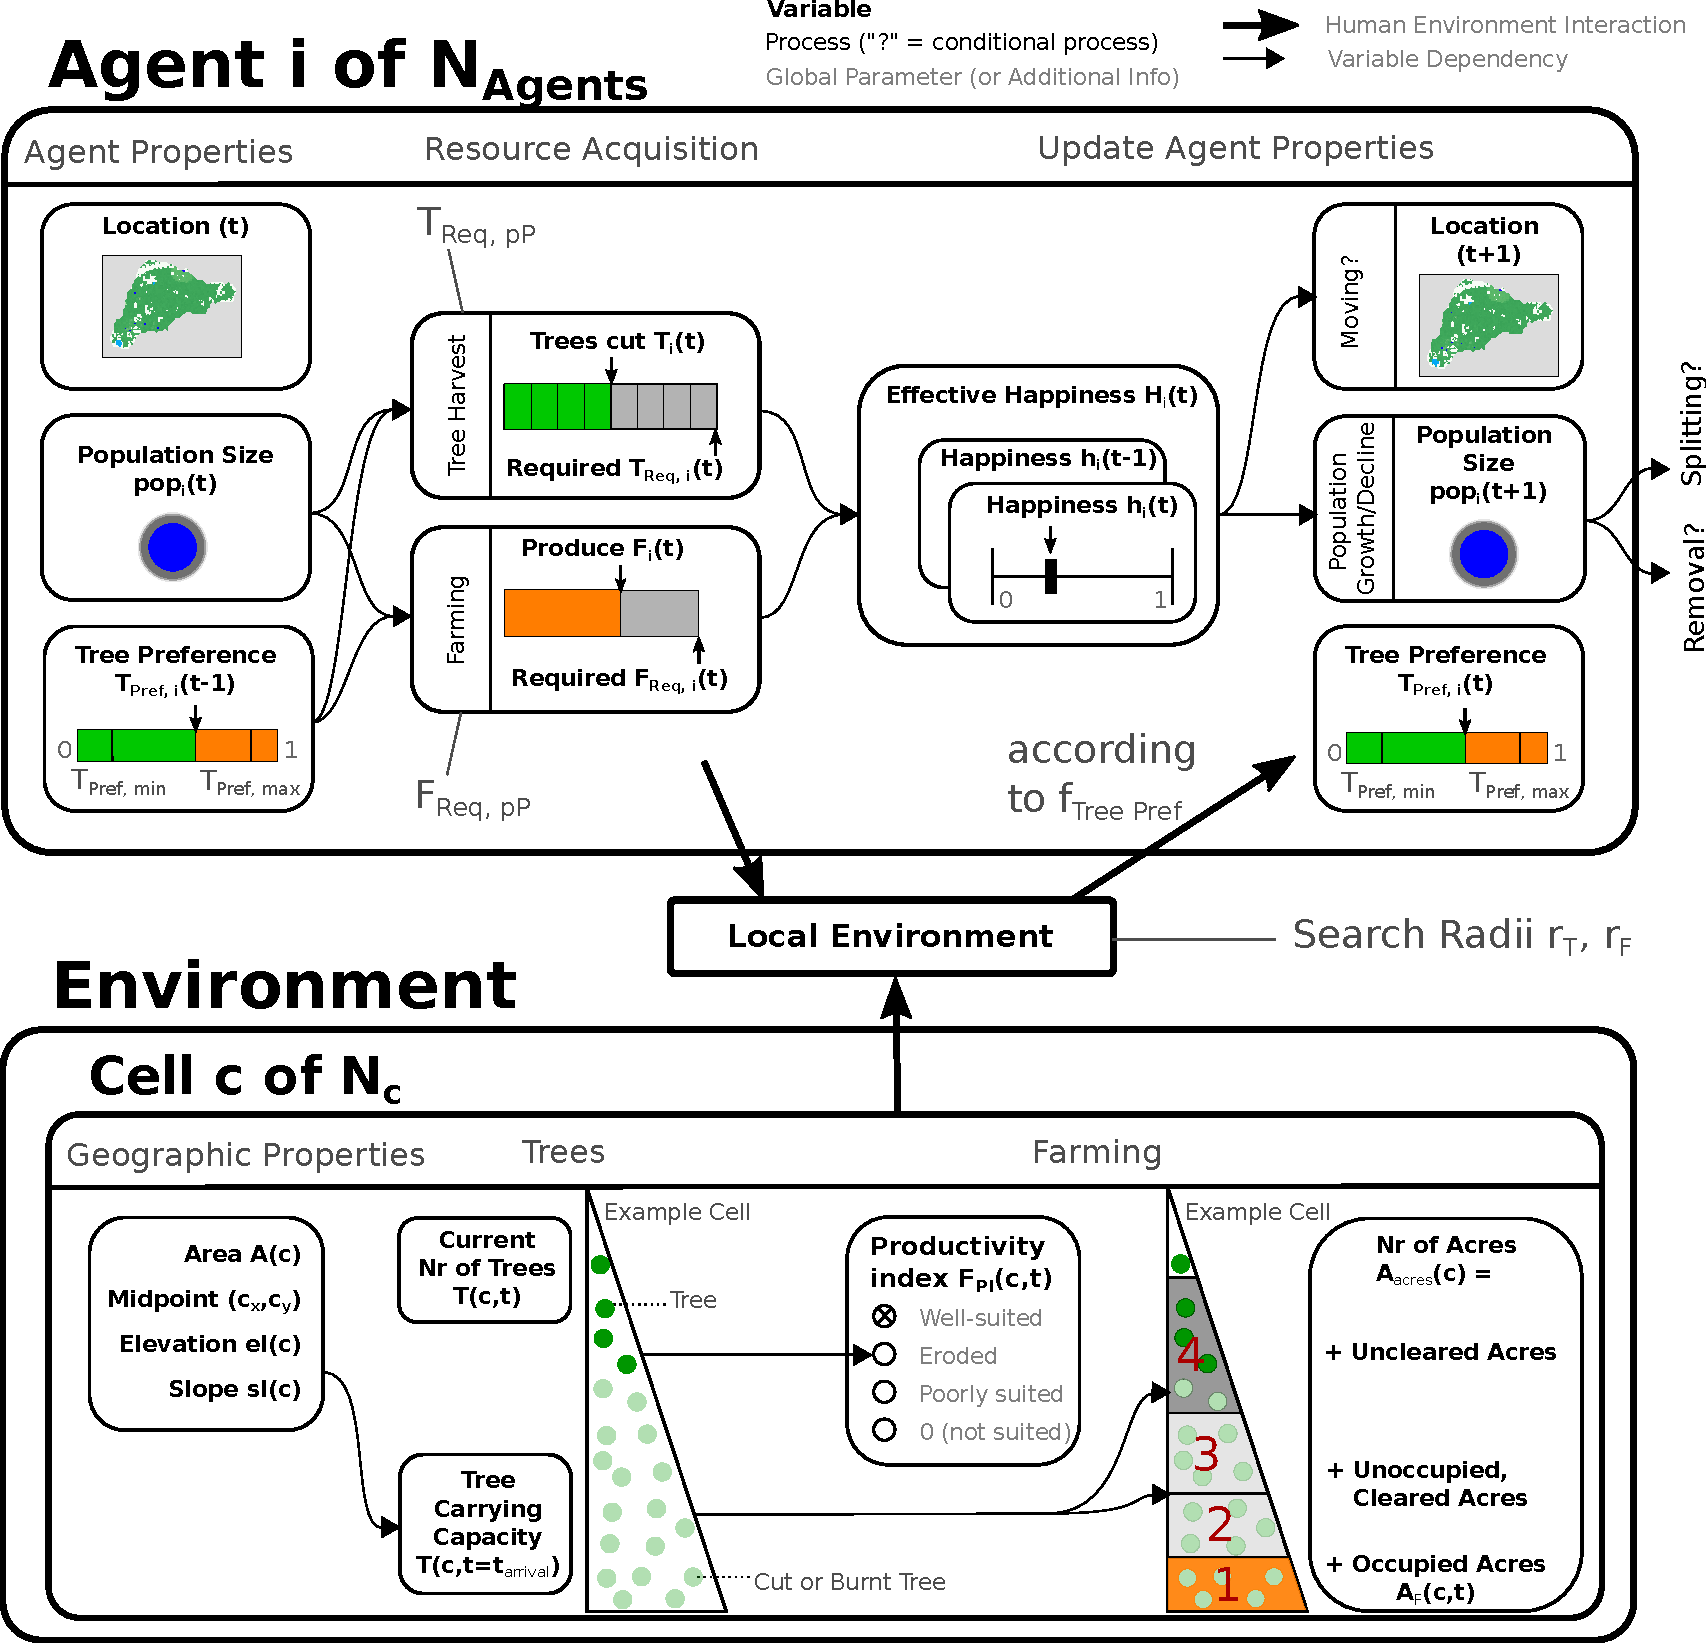
\includegraphics[width=1.\textwidth, center]{images/SketchABM2/sketch_triangles.pdf}
	\caption{
		Sketch of an update of agent $i$.
		The environment consists of $N_\text{c}$ discretised cells (triangles), $c$, with certain geographic properties: Area $A(c)$, midpoint $\vec{c}$, terrain elevation $el(c)$, and slope $sl(c)$.  %population density $\frac{pop(C_\text{F}(t)}{r_\text{F}^2\pi}$) (within cells in a circle with radius $r_{\rm F}$, $C_{\rm F}(c)$) 
		A cell has two `resource stocks':
		The first is the number of trees $T(c,t)$, with a maximum of the cell's carrying capacity (and initial state) $T(c,t=t_{\rm arrival})$, which depends on $el(c)$ and $sl(c)$. 
		The second is the number of arable sites, $A_\text{acres}(c)$ with each site having a basic unit area of $1\, {\rm acre}$, consisting of (1) uncleared, (2) cleared but unoccupied, and (3) occupied sites and the corresponding Farming Productivity Index, $F_{\rm PI}(c,t)$, of the cell.
		Agent $i$ represents a household with a settlement location $(x_\text{i},\, y_\text{i})(t)$ (corresponding cell $c_\text{i}(t)$), a population size $pop_\text{i}(t)$, and a tree preference $T_\text{Pref, \, i}(t-1)$, reflecting the state of the local environment in the previous year. The latter two (together with global, tunable per person resource requirement constants, $T_{Req, \, pP}$ and  $F_\text{requ, \, pP}$) determine the agent's requirements for tree cutting, $T_\text{Req, \, i}(t)$ and farming, $F_\text{Req, \, i}(t)$, each year.
		If the location of the agent allows open-ocean fishing, the farming requirement, $F_\text{Req, i}(t)$ is immediately fulfilled without occupying arable sites.
		The success of the resource acquisition, $T_{\rm i}(t)$ and $F_{\rm i} (t)$, given the local environment (characterised by resource search radii $r_{\rm T}$ and $r_{\rm F}$) then determines the current and effective happiness of the agent, $h_{\rm i}(t)$ and $H_{\rm i}(t)$. %requirements depends on the resource stocks of cells in radii $r_{\rm T}$ for tree harvest and $r_{\rm F}$ for farming. 
		The latter then determines the agent's population dynamics (including potential splitting or removal of the agent) and potential relocation of the settlement (according to a semi-rationale decision making process sketched in Figure \ref{fig:sketchmoving}).
		Finally, the tree preference, $T_\text{Pref, i}(t)$ is updated according to a function $f_{\rm Tree \ Pref}$ of the change of the local environment.
	}
	\label{fig:SketchABM}
\end{figure}

\FloatBarrier
\section{A Discretised Map of Easter Island with Geographical and Biological Features}\label{sec:CreateMap}
\paragraph{Map Discretisation.}
I create a discretised map dividing the island into a number of small 2D triangular cells with certain geographical features.
First, I define an equidistant grid on Easter Island\footnote{Ranging $18\, {\rm km}$ in latitudinal (from $-27.2050^\circ N$ to $-27.0437^\circ N$) and $24\, {\rm km}$ in longitudinal direction (from  $-109.4650^\circ E$ to 
 $-109.2227^\circ E$)} with a grid size of $\delta_{\rm x} \approx 320\, {\rm m}$ between points in $x$- (i.e.\ $75$ points) and $\delta_{\rm y} \approx 360\, {\rm m}$ in y-direction (i.e.\ $50$ points). 
In principle, the map can be created with any arbitrary resolution, constrained only by the resolution of the underlying geographical data. 
Also other grid types, e.g.\ with adaptive $\delta_{\rm x,y}$ to focus on regions of interest, are compatible with the model. 
While a higher resolution increases detailed geographical representation and reduces discretisation errors, computation time of the presented model scales highly non-linearly (see Section \ref{sec:Moving}).
Hence, a trade-off has to be found between detail or accuracy and computation time.
Next, I create 2D triangular cells from this grid using \textit{matplotlib}\footnote{\citet{matplotlib}}'s Delaunay triangulation package.
A cell $c$ is characterised by its midpoint $\vec{c} = (c_{\rm x},\, c_{\rm y})$. 
Since all cells are Delaunay triangles, their smallest angles are maximised and the midpoint, $\vec{c}$, provides a reasonable representation of the cell.
%Topic: Define Easter Island
%Using geographical information, the triangles making up Easter Island are selected.
Features of the terrain, elevation, $el(c)$, and slope, $sl(c)$, of Easter Island are obtained from a publicly available, high resolution elevation map \citep{Jarvis2008CIGAR} via the Google Earth Engine interface\footnote{\citet{gorelick2017google}} and evaluated at the corresponding midpoint $\vec{c}$.
All cells located on the ocean (i.e.\ $c$ with $el(c)=0$) are masked out and discarded.
The cells corresponding to the island's three small crater lakes are also identified.
The remaining cells constitute the landmass of the discretised island, which can be settled, deforested or farmed by the agents. 
With the resolution given above, a total of $N_{\rm c} = 2768$ cells are considered with an area of roughly $A(c)= 0.06 \, {\rm km^2}$ each.
The total area of the obtained discretised Easter Island map is $A=159.2\, {\rm km^2}$, ($163.6\, {\rm km^2}$ in reality) providing a detailed, cellular representation of geographical features (location $\vec{c}$, area $A(c)$, elevation $el(c)$, and slope $sl(c)$).

%There are three -- or two in periods of major droughts (see \citet{Rull2020}) -- permanent crater lakes on Easter Island, providing the major freshwater sources for the prehistoric Easter Island population, as discussed later in Section \ref{sec:Moving}.
%The corresponding cells are calculated from the locations and radii of these lakes. 
%This procedure gives a detailed, discretised representation via triangular cells with geographical features of Easter Island. 
 
%Archaeological records indicate that crater lakes could have dried out during major drought periods.
%In particular the drying of Rano Raraku in the East of Easter Island during the Medieval Climate Anomaly ($500-1200 \, \rm{A.D.}$) and during the Little Ice Age ($1570-1720\, \rm{A.D.}$) \citep{Rull2020} and the consequences have been a reoccuring theme of scientific debate (e.g.\ \citet{Cauwe2011}). 
%Such drought events can be simulated by removing each of the lakes for some period of time from the map.

\paragraph{Trees.}
%Next to purely geographical, each cell has characteristic biological features, trees and .% next to the geographic specification before. 
Each cell $c$ on the discretised map contains a number of trees, denoted as $T(c,t)$ (or tree density $T(c,t)/A(c)$).
%While the assumption of constant climatic conditions throughout Easter Island's history has been challenged recently \citep{Rull2020}, I only consider anthropogenic deforestation $T(c,t)$.
The island's forest system is assumed to be in equilibrium at the time of the arrival of the first settlers, $t_\text{arrival}$, and, thus, $T(c,t=t_\text{arrival})$ is the constant carrying capacity of palm trees for each cell $c$ on the island (c.f.\ \citen{Brander1998}).
There is is still some uncertainty about the total number and spatial patterns of palm trees at $t=t_\text{arrival}$.
\citet{Mieth2015} estimated a total of $16\cdot 10^6$ trees covering $80\%$ of the island from observed root casts in the soil, whereas e.g.\ \citet{Brandt2015} initialise the model with a conservative estimate of $8\cdot 10^6$ trees. 
Most studies assume an island wide, dense distribution of the palm trees. 
E.g.\ \citet{Bahn2017} stated that soil sufficient for tree growth is present `almost everywhere on the island, apart from the steepest parts of the cliffs and the youngest lava surfaces' (i.e.\ the highest elevations of Mount Terevaka). 
However, \citet{Rull2020} also investigated the possibility of variable, mosaic vegetation patterns with high densities of trees around the lakes and the coastal areas.
%As mentioned in the introduction \TODO, there's no comprehensive record of tree patterns. While some \todo{cite Rull?} archaeologsits state that the majority ($80\%$ of the island) was densley forrested \todo{cite}. 
The model presented here can incorporate any pattern of pre-arrival tree density. 
For this thesis, I assume a total\footnote{Bold symbols denote iterations over all cells (or agents) in the thesis.} of 
%by two terrain-dependent tree density levels: (1) `normal density' for low elevation $el(c)<250\, \rm{m}$ and slope $sl(c)<5^\circ$, (2) `half density' for moderately high elevations $250\, \rm{m}el(c)<430\, \rm{m}$ (elevation of Lake Rano Aroi) and slope $5^\circ < sl(c) < 9^\circ$, and (3) `zero density' for cells above these thresholds.
\begin{equation}
\mathbf{T}(t=t_\text{arrival}) = \sum_{c} \, T(c,t=t_\text{arrival}) =  16 \cdot 10^6 \, \text{trees}
\end{equation} 
trees distributed according to an equal density pattern excluding those cells with very high elevation or slope ($el(c)>450\, {\rm m}$ or $sl(c)>10^\circ$ $\Rightarrow$ $T(c,t) = 0$).
% with uniform probability among all cells with potential for tree growth. 
A resulting map of pre-arrival tree numbers $T(c,t_\text{arrival})$ in cells $c$ extending on $86\%$ of Easter Island is shown in Figure \ref{fig:Map_tree}.

\begin{figure}
	\centering
	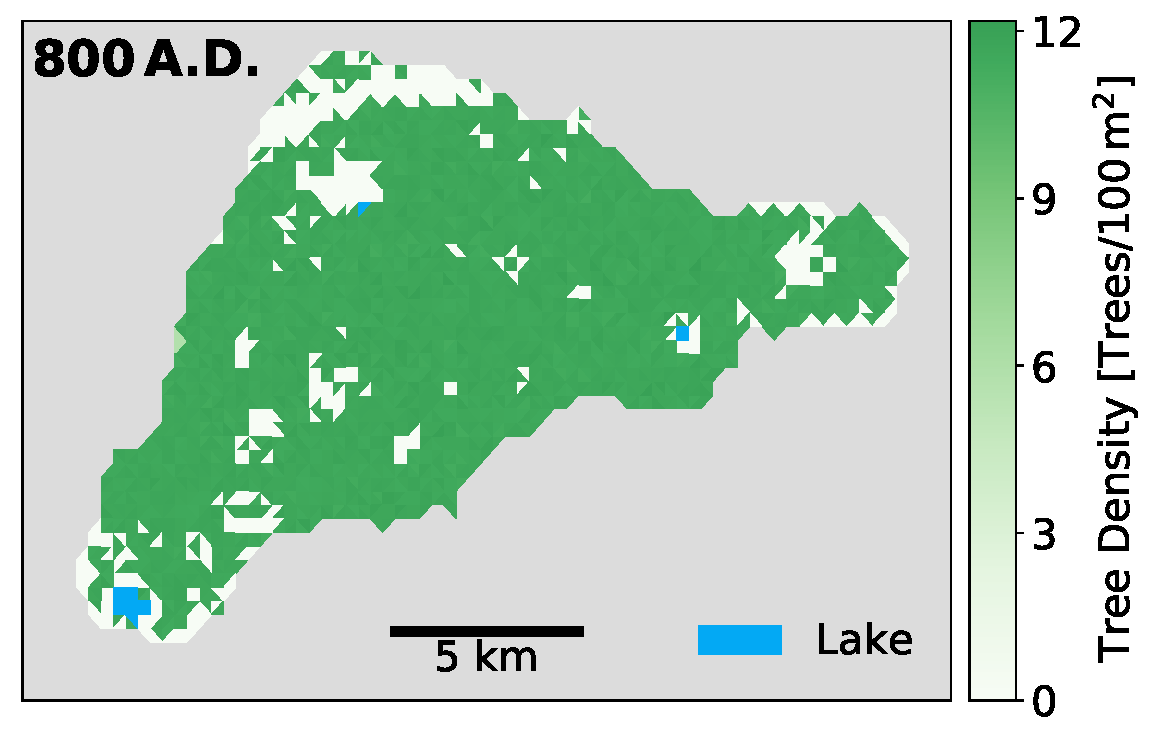
\includegraphics[width=0.7\textwidth]{images/map_carrCap.pdf}
	\caption{The tree density in each cell at carrying capacity (prior to the arrival of the first settlers), $T(c,t_\text{arrival})/A(c)$.}
	\label{fig:Map_tree}
\end{figure}

\paragraph{Tree Dynamics.}
Through anthropogenic deforestation, the variable tree number in each cell, $T(c,t)$, declines.
Natural removal (e.g.\ through a changing climate) is not considered in the model.
%As described in the Introduction, the impact of the human deforestation compared to the invasive Polynesian rats on the environmental degradation of the island is debated (e.g.\ \citet{Bahn2017} and \citet{Hunt2007}).
In the literature on Easter Island, there seems to be a consensus between the two major contrasting theories that rats effectively hindered tree regrowth by feeding on palm nuts (e.g.\ \citen{Bahn2017}; \citen{Hunt2007}).
In line with this argument, forest regeneration does not occur in the standard configuration of this model.
Trees, therefore, constitute an entirely non-renewable resource in this setting. 
However, I also conduct alternative experiments, in which the forest can hypothetically regenerate following anthropogenic deforestation.
In this alternative setting, each year, tree numbers $T(c,t)$ in all cells $c$ regrow logistically to their (local) carrying capacity $T(c,t=t_\text{Arrival})$ if there is no farming activity on the specific cells.
The maximum growth rate of the palm trees is believed to be rather slow and has even been made responsible for the ecological collapse of the island by \citet{Brander1998}.
%Hence, in the alternative experiments, I set the maximum logistic tree regeneration growth rate to
Here (in the alternative scenario), I use
\begin{equation}
g_{\rm T} = 0.05\, {\rm \frac{1}{yr}} \ ,
\end{equation}
based on the estimated maximum tree regrowth rate in \citet{Brandt2015}, i.e.\ between $0.02$ and $0.07\, {\rm \frac{1}{yr}}$ in the absence of rats.
Some cells are deforested entirely in a single update step, which disables logistic regeneration. 
However, with seeds being transported to the empty cell e.g.\ through wind, birds or human activity, forests regrow even in empty land.
To incorporate this, a small number of trees `pops up' ($0.5\%$ of the cell's carrying capacity) after a treeless cell has been left barren, i.e.\ without any farming activity, for $10$ consecutive years.
In summary, in this environmental model the tree number in a cell $c$ either does not regenerate at all, i.e.\ 
\begin{equation}
T(c,t+1) \stackrel{\text{`without'}}{=} T(c,t)
\end{equation}
(not considering the anthropogenic deforestation) or alternatively regenerates as
\begin{equation}\label{eq:treeupdate}
T(c,t+1)\stackrel{\text{`with'}}{=} \begin{cases}
T(c,t) + T(c,t) \cdot g_{\rm T} \cdot \left(1- \frac{T(c,t)}{T(c,t_{\rm Arrival})}\right) \quad & \forall \ c \text{ with } A_{\rm F}(c,t)=0 \\
0.005 \cdot T(c,t_{\rm Arrival})  & \forall  \ c \text{ with } T(c,t)=0 \text{ and}\\
& A_{\rm F}(c,\hat{t})=0 \  \ \forall \  \hat{t} \in \{t-10, \ldots, t\} \\
0 & \text{ else }
\end{cases}
\end{equation}
where $A_{\rm F}(c,t)$ is the number of occupied sites in cell $c$ at any given time. 
These two scenarios, labelled as `without' and `with' forest regeneration, allow for testing of the impact of the Polynesian rats, assuming that they effectively hindered tree regeneration.

\paragraph{Farming Sites.}
Next to the resource trees, the environment also provides land for active farming of sweet potatoes\footnote{Sweet Potato was the dominant staple crop on Easter Island (at least in later phases) \citep{Louwagie2006}} as a renewable, second resource (similar to the model of \citen{dAlessandro2007}).
A single farming site on arable land has a constant, basic unit area of $1\, {\rm acre}$ on a cell. 
%Hence, if a cell is arable, it provides the possibility for 
%$A_{\rm acres}(c)$ farming sites to be occupied by an agent,
%which is the the area of the cell, $A(c)$, in acres rounded down.
Hence, with an average area of $0.06\, {\rm km^2} = 14.2\, {\rm acre}$ given the resolution used in this thesis, an arable cell allows typically for $A_{\rm acres}(c)=14$ farming sites.
%The number of occupied sites in each cell is denoted as $\mathbf{A}_{\rm F} (c, t)$.
%\begin{equation}\label{eq:occupied}
%\mathbf{A}_{\rm F} (c, t)  = \sum_{j \in N_{\rm Agents}(t)} \, \sum_{a \, \in \, A_\text{F, j}(t)} \, \delta(a=c)
%\end{equation}
%\todo{Occupied Sites Here}
Such an occupied site provides a constant farming output of crop yield for the agent each year. 

\paragraph{Farming Productivity Index.}
The farming productivity per area, i.e.\ the potential crop yield, is strongly location dependent.
Here, I define a (relative) Farming Productivity Index, $F_\text{PI}(c)$, for each cell $c$ (shown in Figure \ref{fig:Map_agric}). 
While the total potential of farming productivity remains uncertain (as described in the Introduction), some studies used agricultural modelling based on elevation, climate and soil quality data to obtain a more detailed, spatially explicit classification of the farming suitability:
%identified arable sites by using data on rain, climate, temperature, elevation and soil quality in agricultural models (e.g.\ \citet{Louwagie2006} and \citet{Puleston2017}).
%A farmed acre yields a produce according to a (relative) Farming Productivity Index, $F_\text{PI}(c)$.
%The absolute productivity of a well-suited acre in units of people it can support is taken from calculations in \citet{Puleston2017} assuming two different Nitrogen fixation scenarios (see in detail later).
%The map of Farming Productivity Indices $F_\text{PI}(c)$ of all cells on Easter Island is shown in Figure \ref{fig:Map_agric}, thus defining where agents have access to farming and how productive farming would have been in this location in the model. 
%Topic: Agriculture Yield
%\paragraph{Studies on the Farming Quality}
%The Easter Island society also cultivated renewable staple crops as an alternative to harvesting the non- or slowly renewable resource, tree\citep{dAlessandro2007}.
%Hence, agents in this model also farm on arable land in a two resource dependency similar to previous models \citep{dAlessandro2007}.
%Agents in this model transfer arable land into farming sites, in particular for sweet potato cultivation, the dominant staple crop on Easter Island (at least in later phases) \citep{Louwagie2006}.
%As described in the Introduction, Easter Island's suitability for farming, especially w.r.t.\ climate and soil, has been subject to excessive debate.
%While the total potential of agricultural productivity remains uncertain, several studies identified arable sites by using data on rain, climate, temperature, elevation and soil quality in agricultural models (e.g.\ \citet{Louwagie2006} and \citet{Puleston2017}).
\begin{itemize}
	\item \citet{Puleston2017} created a map (Figure 4 in the publication) 
	indicating regions that meet a certain viability criterion for sweet potato cultivation.
	This criterion marks $19\%$ of the island as agriculturally viable, mainly in the lowland, coastal region.
	In this model, I denote all cells of the discretised map, which are located in this region `well-suited' and assign a high farming productivity index $F_{\rm PI}|_{\rm well}$.
	Additionally, the map reported by \citet{Puleston2017} includes areas that did not meet the criterion but in which small, patchy areas of agricultural structures were identified from satellite images. 
	Consequently, the yield from these regions must have been low such that the farmers used techniques like labour intensive, large-scale lithic mulching, which mainly increased moisture availability, and efficient crop management, e.g.\ plant spacing and frequent fallowing \citep{Louwagie2006}.
	I call all cells in this region `poorly suited' and assign a low farming productivity index $F_{\rm PI}|_{\rm poor}$.
	\item \citet{Louwagie2006} developed a classification for successful cultivation of several crops based on climate and soil property measurements at a few sites on the island and assigned relative yields to these sites. 
	The majority of the measurement sites located at the foots of smaller craters along the arable coasts correspond partly with the well-suited and partly the poorly suited regions\footnote{Comparing roughly Figure 1 of \citet{Louwagie2006} with Figure 4 of \citet{Puleston2017}.}. For most climatic conditions these were classified as mostly `marginally to moderately suitable' for sweet potato cultivation (corresponding to a relative yield of around $55\%$ $(20-80\%)$ of an optimal farming site) and, especially in wet years, some locations were classified as `highly suitable' (relative yield of $>80\%$).
	One of the studied sites (`Vaitea'), located in the poorly suited region, was found `not suitable' for farming due to insufficient nutrition availability (relative yield of $0-20\%$) despite archaeological evidence of gardens in this area.
	Based on these results, which provide the best estimate available, I choose
	\begin{eqnarray*}
		F_\text{PI}|_\text{well} & = 80\% & \text{ for well-suited (highly to moderately suitable)}\\
		F_\text{PI}|_\text{poor} & = 10\%  & \text{ for poorly suited (not suitable)}\\
		F_\text{PI}|_\text{non-viable} & = 0\% & \text{ for non-viable sites}
	\end{eqnarray*}
	depending on a cell's classification by \citet{Puleston2017} into well-suited and poorly suited cells.
	Hence, the total resulting arable land area in this model (shown in Figure \ref{fig:Map_agric}) is ca.\ $29\,  {\rm km^2}$ (i.e.\ $18\%$ of the total island area) for well-suited sites and, additionally, $50\, {\rm km^2}$ (i.e.\ $31\%$ of the total island area) for poorly suited sites with low Farming Productivity Index.
	%However, only a small, patchy fraction of this `poorly suited' region was actually effectively farmed as estimated by \citet{Puleston2017} by identifying agricultural structures from satellite data. 
	% also indicating that there is a strong difference between well-suited sites and those
\end{itemize}

%\paragraph{Map of Arable Land}
%In order to obtain a spatially explicit differentiation between arable and non-arable land, I use a map created by \citet{Puleston2017} (Figure 4) indicating regions meeting a certain viability criterion for sweet potato cultivation.
%This criterion %is based on an agricultural model of climate data and soil quality and 
%marked $19\%$ of the island as agriculturally viable, mainly in the lowland, coastal region.
%However, widespread systems of gardens were also found in the upland regions classified as non-viable by \citet{Puleston2017}.
%The authors state that these gardens added only a small fraction of actually farmed land to the viable region, though.
%Here, I use three levels of viability for the discretised map: 
%%A cell is either `well-suited' if located in the viable region, `poorly suited' if located in the non-viable region which was nevertheless farmed, or `non-viable' else (cp.\ with \citet{Puleston2017} (Figure 4)).
%
%The difference between well-suited and poorly suited arable land is reflected in the Farming Productivity I
%
%
%The total resulting arable land area in this model (shown in Figure \ref{fig:Map_agric}) is ca.\ $29\,  {\rm km^2}$ (i.e.\ $18\%$) for well-suited sites and, additionally, $50\, {\rm km^2}$ (i.e.\ $31\%$) for poorly suited sites.
%%This fraction of arable land is in line with several different estimates from e.g.\ \TODO \citet{Bahn2017}???
%%. TODO SOMEONE SAID THAT 50\% of the land was cultivated?
%
%\paragraph{Farming Productivity Indices}
%I distinguish well-suited from poorly suited cells by assigning different dryland Farming Productivity Indices, $F_\text{PI}(c)$, to associated cells.
%\citet{Louwagie2006} developed a classification for successful cultivation of several crops based on climate and soil property measurements at a few sites on the island and assigned classes of relative yields to them. 
%One of the studied sites (Vaitea), which coincides with the poorly suited region in \citet{Puleston2017}\footnote{Compare Figure 1 of \citet{Louwagie2006} with Figure 4 of \citet{Puleston2017}.}, was found not suitable for farming due to insufficient nutrition availability (with a relative yield of $0-20\%$ compared to an optimal site) despite archaeological evidence of gardens in this area.
%To enhance yields, the islanders used techniques like labour intensive, large-scale lithic mulching, which mainly increased moisture availability, and efficient crop management, e.g.\ plant spacing and frequent fallowing \citep{Louwagie2006}.
%The per area productivity, however, remains low even with these techniques in place with nutrient availability being the main constraint as also implied by the analysis in \citet{Puleston2017}.
%The other sites in \citet{Louwagie2006} located at the foots of smaller craters along the arable coasts, were classified as mostly `marginally to moderately suitable' for sweet potato cultivation for most climatic conditions with some locations showing `high suitability' (relative yield $>80\%$) especially in wet years. 
%These sites are mainly located in the well-suited or poorly suited regions of the map in \citet{Puleston2017}.
%Hence, following roughly the classification by \citet{Louwagie2006}, a Farming Productivity Indices, $F_\text{PI}(c)$ is assigned to each cell (and its corresponding sites)
%\begin{eqnarray*}
%	F_\text{PI}|_\text{well} & = 80\% & \text{ for well-suited (highly to moderately suitable)}\\
%	F_\text{PI}|_\text{poor} & = 10\%  & \text{ for poorly suited (not suitable)}\\
%	F_\text{PI}|_\text{non-viable} & = 0\% & \text{ for non-viable sites}
%\end{eqnarray*}
%depending on its classification by \citet{Puleston2017} into well-suited and poorly suited cells.

\paragraph{Erosion.}
Soil erosion through radical deforestation and heavy rainfalls degraded the farming productivity of Easter Island especially in the later phase (e.g.\ \citen{Brander1998}; \citen{Mieth2005}; \citen{Bahn2017}).
As trees are removed from a region, rain can wash away nutrient-rich soil and reveal less fertile ground with reduced relative yield. % \citep{Mieth2005}.
In the model, I assume that, if a well-suited cell is entirely deforested, the land erodes and, thus, the cell's $F_\text{PI}(c)$ reduces to 
\begin{equation}
F_\text{PI}|_\text{eroded}=50\% \quad \text{for well-suited cells with } T(c,t)=0 \ .
\end{equation}
This soil degradation is reverted as soon as trees pop back up (i.e.\ if the cell has been kept barren (without farming) for $10$ years as described in equation \ref{eq:treeupdate}).


\begin{figure}
	\centering
	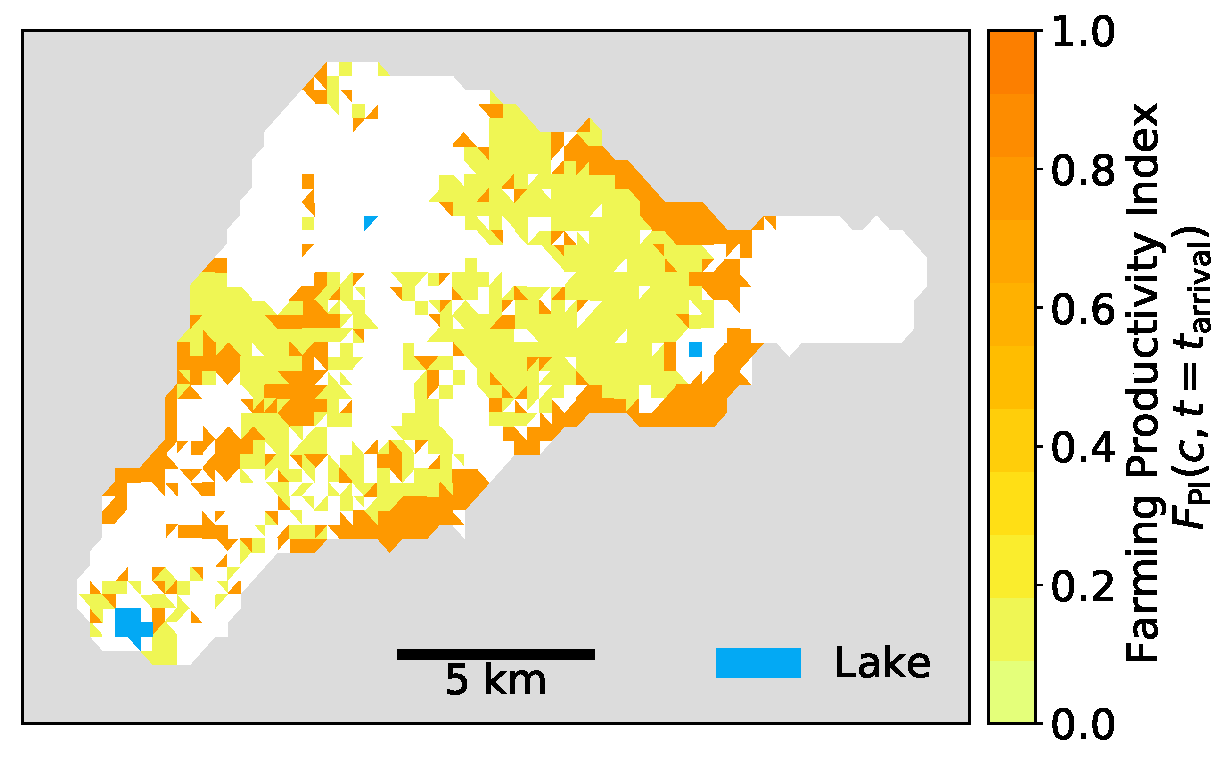
\includegraphics[width=\textwidth]{images/Plot_F_PI_c.pdf}
	\caption{A map of the (sweet potato) Farming Productivity Indices, $F_\text{PI}(c)$, in each cell of the discretised map of Easter Island. The model makes use of the map of \citet{Puleston2017} classifying arable land into viable areas (here `well-suited sites'), non-viable but nevertheless partially farmed (here `poorly suited sites'), and non-viable sites derived from an agricultural model of climate and soil quality. 
	This classification is combined with measurements of land suitability in several sites \citep{Louwagie2006} giving rise to a simple, spatially explicit map of farming potential parametrised by the Farming Productivity Index $F_\text{PI}(c)$.}
	%The Farming Productivity Indices in areas where gardening was observed but that did not meet the agricultural potential of \citet{Puleston2017}'s criterion is $10\%$ in line with the result of a model of agricultural yield from measurments in one such site by \citet{Louwagie2006}.}
	\label{fig:Map_agric}
\end{figure}


%\section{Agent Properties and Agent-Environment Interaction}\label{sec:AgentUpdate}
% Topic: Agents Households with properties
\FloatBarrier
\section{Human Agents and their Features}\label{sec:agentprops}
\paragraph{Basic Variables.}
The ABM consists of a variable number of agents, $N_{\rm Agents}(t)$, which represent households, situated on the discretised map derived in Section \ref{sec:CreateMap}.
An agent with index $i$ has several features describing its state at time $t$:
The settlement is located at 
\begin{equation}
	\vec{x_{\rm i}}(t) = (x_{\rm i},\, y_{\rm i})(t)
\end{equation}
 on the discretised map and, hence, associated with one specific cell $c_{\rm i}(t)$.
 The agent's population size, i.e.\ the number of individuals in the household, 
 \begin{equation}pop_{\rm i}(t) \end{equation}
typically ranges from $12$ to about $42$. % ranging from $6$ to $42$ .
Macroscopic island-wide aggregate variables, like population size, are simply obtained by summation over all agents, which I denote with bold symbols (equivalent to summation over cells). 
%Iterations over all agents (or cells of the map for the corresponding variables) are denoted via bold symbols in all equations in this thesis.

\paragraph{Resource Search Radii.}
Agents have access to two different types of resources, trees (and consequent derivate products) and farmed products, by interacting with their local environment defined by fixed resource search radii.
%An agent $i$ harvests these resources from cells with midpoints
% $\vec{\tilde{c}}$ located within fixed radii of the agent's settlement:
Hence, the local environment of agent $i$ is defined as:
\begin{equation} \label{eq:Circle_T}
C_{T}(x_{\rm i}(t)) = \{ \tilde{c}\ | \   | |  \vec{\tilde{c}} - \vec{x_{\rm i}}(t) | |  \leq r_{\rm T} \} 
\end{equation}
for the resource tree with search radius $r_{\rm T} =2\, {\rm km}$ and 
\begin{equation} \label{eq:Circle_F}
C_{F}(x_{\rm i}(t)) = \{ \tilde{c}\ | \   | |  \vec{\tilde{c}} - \vec{x_{\rm i}}(t) | |  \leq r_{F} \}
\end{equation}
for occupying farming sites with radius $r_{\rm F} = 1\, {\rm km}$.

\paragraph{Tree Preference.}
The agent's total required resource uptake is split between tree cutting and farming yield, given by a trait parameter, the tree preference $T_\text{Pref, i}(t)$ for agent $i$ at time $t$, which reflects the state of the local environment.
%Changes in the tree preference are an adaption of the agent's harvest behaviour to changes in its local environment.
In the first phase of settling on the island, the civilisation mainly lived off the island's abundant natural resources (here trees) \citep{Bahn2017}.
However, over time, the economy `switched from predominantly hunter-gatherer to a dryland farming society' \citep{Louwagie2006}.
%In the model, this behavioural shift is expressed as a decrease in the variable tree preference parameter, $T_\text{Pref, i}(t)$ of each agent over time.
The tree preference trait, $T_\text{Pref, i}(t)$, in this model is designed such that agent's adjust their harvest behaviour for next year given the current state of the local environment (in particular the level of deforestation).
%Changes in the tree preference are an adaption of the agent's harvest behaviour for next year to changes of the state of its local environment (in particular the level of deforestation).
%It is an adaptive trait reflecting the local state of the environment around an agent, in particular the local abundance of trees. %(i.e.\ trees $T(c,t)$ of cells within $C_{\rm T}(c_\text{i}(t)$).
Hence, as trees are removed from an agent's local environment and more arable land is cleared freeing up space for agriculture, the agent's tree preferences decrease and its farming requirement increases accordingly.
%This tree preference indicates the value of tree harvest over agricultural production and, hence, increases the need for one over the other in order to fill the resource requirements.
%The tree preference is high in the initial state, but decreases as trees become scarce and more land is available for cultivation of crops.
%Hence, $TPref_{\rm i}(t)$ responds to some degree to the local environment of the agent.
%In this model, $T_\text{Pref, i}(t)$ depends on the local, relative change of tree density within the tree search radius $r_{\rm T}$ with respect to the initial state at $t=t_\text{arrival}$, i.e.:
In this model, $T_\text{Pref, i}(t)$ depends on the relative change of tree density with respect to the initial state at $t=t_\text{arrival}$ in the local environment:
\begin{equation}\label{eq:TPref}
T_\text{Pref, i}(t) = f_\text{Tree Pref}\left( \, \frac{\sum_{\tilde{c} \in C_{T}(c_{\rm i}(t)) } \, T(\tilde{c}, t)}{\sum_{\tilde{c} \in C_{T}(c_{\rm i}(t))} \, T(\tilde{c}, t_\text{arrival}) } \, \right)
\end{equation}
The shape of the function $f_\text{Tree Pref}$ is an indicator of the adaptation strategy of the economy/society to environmental change. How fast do agents adapt their harvest behaviour, when the non-renewable resources, trees, are depleted?
I consider four strategies (shown in Figure \ref{fig:TPref_T}): The tree preference $T_\text{Pref, i}(t)$ decreases
\begin{itemize}
	\item linearly with the local, relative tree density decline (linear case).  
	\item delayed with the local, relative tree density decline (delayed case).
	\item faster than the local, relative tree density decline (faster or careful case),
	\item first delayed, and at some point faster than the local, relative tree density decline (logistic case) 
\end{itemize}
\begin{figure}
	\centering
	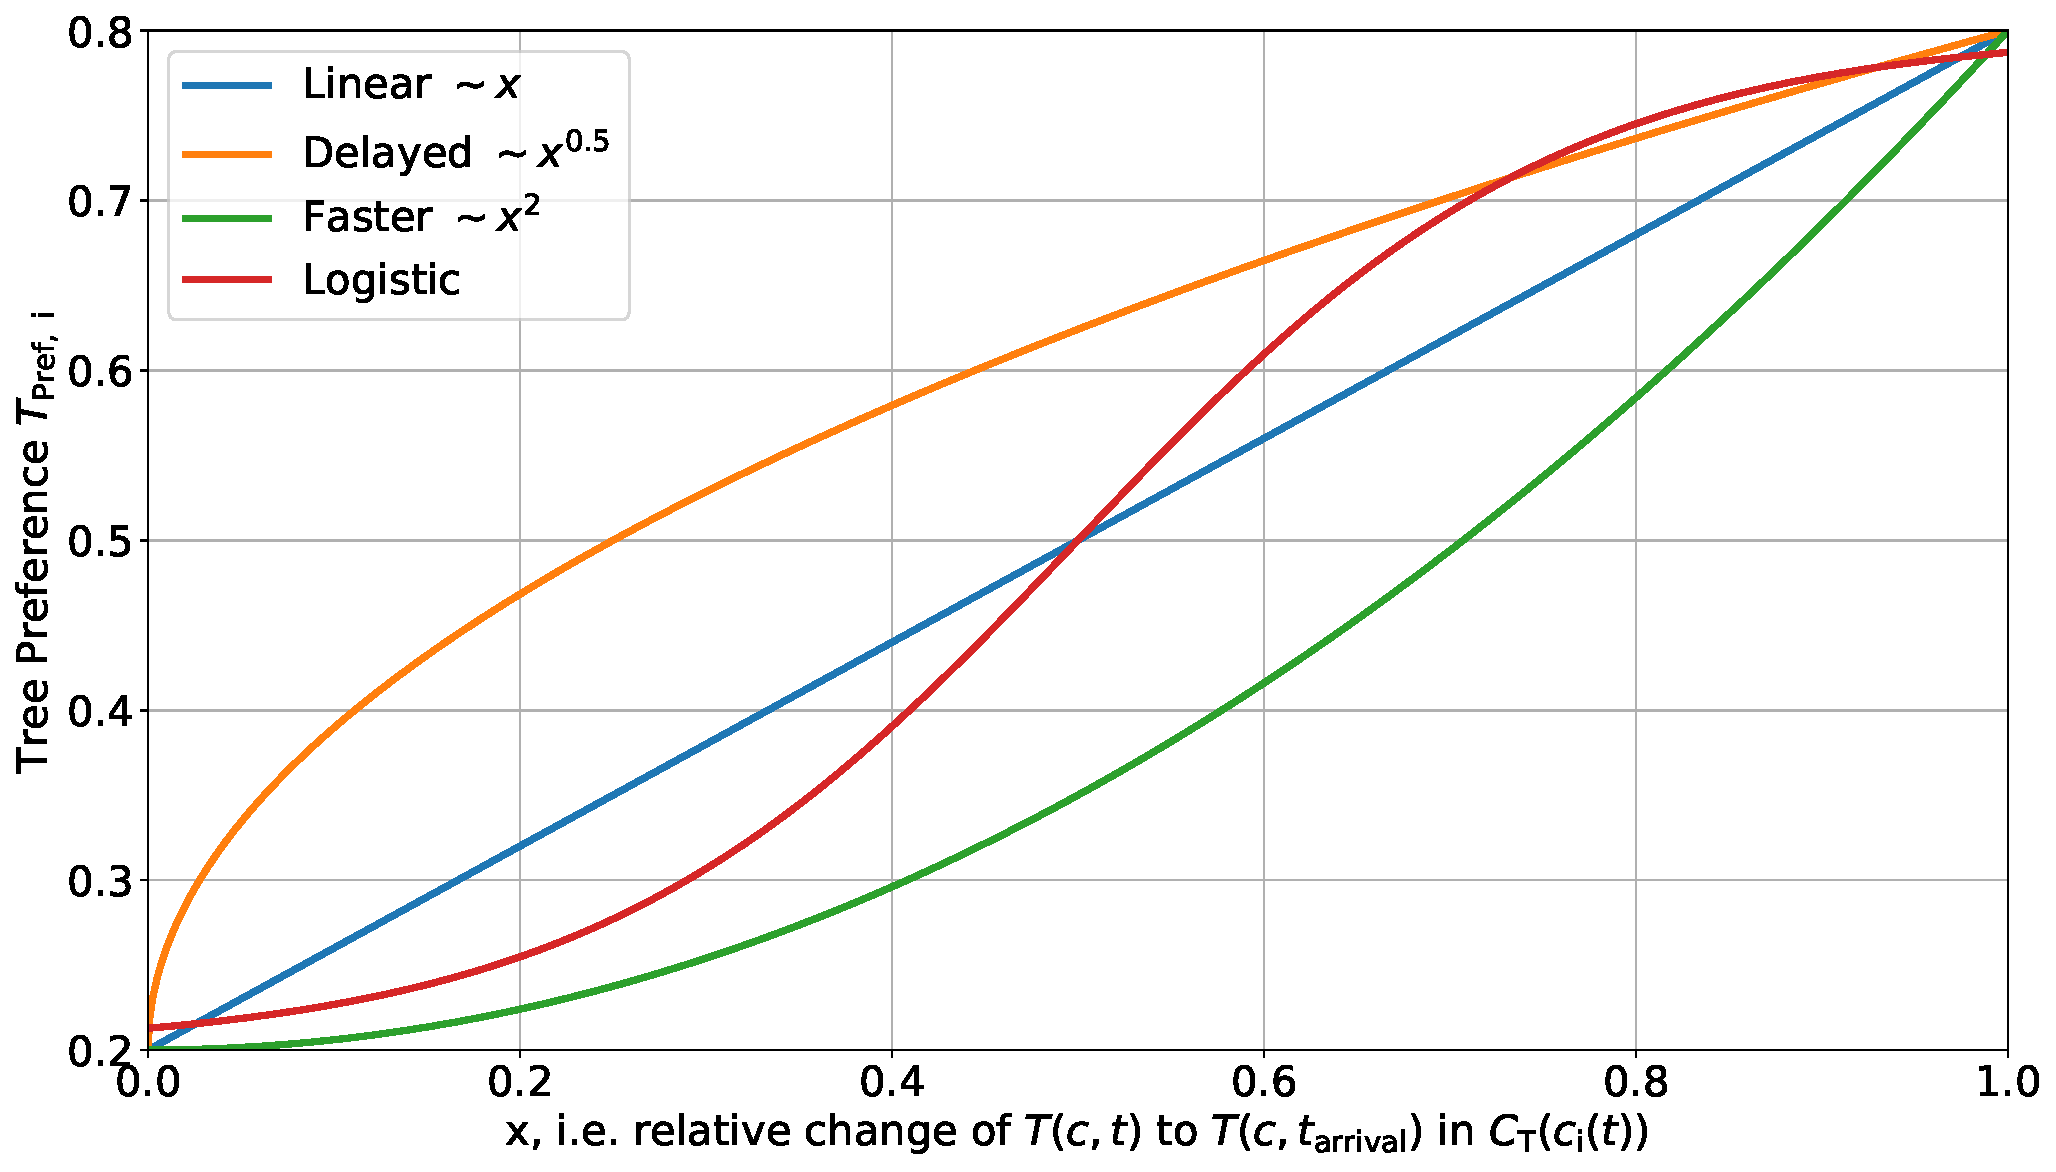
\includegraphics[width=\textwidth]{images/TPref}
	\caption{Relationships of an agent's tree preference, $T_\text{Pref, i}(t)$, with respect to relative changes in local tree density for the four considered adaptive strategies $f_\text{Tree Pref}$ with $x$ given in equation~\ref{eq:TPref}.}
	\label{fig:TPref_T}
\end{figure}
The tree preference is limited to a certain range, assuming an agent can not live purely off trees (and associated derivate products), but, at the same time, some tree cutting is always required even for maximum agricultural production (e.g.\ as cooking wood or for tools). 
Here, I choose: 
\begin{equation}
T_\text{Pref, min} = 0.2 \quad \text{and} \quad T_\text{Pref, max} = 0.8
\end{equation} 
In the standard configuration in this model, I use the linear relation and, hence, 
\begin{equation}
	T_\text{Pref, i}(t) =  \frac{\sum_{\tilde{c} \in C_{T}(c_{\rm i}(t)) } \, T(\tilde{c}, t)}{\sum_{\tilde{c} \in C_{T}(c_{\rm i}(t))} \, T(\tilde{c}, t_\text{arrival}) } \cdot (T_\text{Pref, max}-T_\text{Pref, min}) + T_\text{Pref, min}
\end{equation}
Initially, agents start with maximal tree preference ($T_\text{Pref, i}(t=t_\text{arrival}) = T_\text{Pref, max} \ \  \forall \ i$), which then (in general) decreases slowly as deforestation progresses.

\paragraph{Resource Requirements.}
An agent's required total resource uptake per year increases with the population size and the tree preference calculated after the harvest in the previous year.
Hence, the resource requirements of tree harvest, $T_\text{Req, i}(t)$, and farming produce, $F_\text{Req, i}(t)$, are 
\begin{equation}
T_\text{Req, i}(t) = T_\text{Pref, i}(t-1) \cdot pop_{\rm i}(t) \cdot T_\text{Req, pP} \, 
\end{equation}
and, similarly, 
\begin{equation}
F_\text{Req, i}(t) = (1-T_\text{Pref, i}(t-1)) \cdot pop_{\rm i}(t) \cdot F_\text{Req, pP}\, , 
\end{equation}
where $T_\text{Req, pP}$ is the constant tree requirement per year per person in absence of agriculture and $F_\text{Req, pP}$ is the constant required agriculture production per person in the absence of tree cutting.

%\paragraph{Tree Requirement per Person}
The tree requirement per person (in the absence of farming), $T_\text{Req, pP}$, in principle depends on a multitude of factors and was presumably heterogeneous among agents.
E.g.\ if agents used sugary sap from cut tree trunks as freshwater replacement (as suggested by \citen{Mieth2015}), they would require a much larger number of trees.
Here, I use a constant parameter of 
\begin{equation}
T_\text{Req, pP} = 5\, \frac{\text{Trees}}{\rm person\cdot yr}
\end{equation}
for all agents (for the standard configuration) based on the maximum harvest rate used in \citet{Brandt2015}, about $3$ to $7$ trees per year\footnote{\citet{Brandt2015} use a only half of the initial trees before arrival of the first settlers, though)}. 
However, I also explore a scenario with doubled tree requirement per person per year.
%In the standard run I am using $5$ Trees per Person per year. However, I vary this parameter in a sensitivity analysis (see Section \ref{sec:SensitivityAnalysis}).

%\paragraph{Farming Requirement per Person}
The requirement of farmed land per person (in the absence of tree cutting), $F_\text{Req, pP}$, crucially determines the overall carrying capacity of the human population.
\citet{Puleston2017} simulate the nutritional productivity of farming on well-suited land (as defined in Section \ref{sec:CreateMap}) for two different environmental scenarios of Nitrogen fixation in the soil, i.e.\ the rate at which Nitrogen is renewed, which represents a major uncertainty in their model\footnote{I do not consider fallowing as farming practice to increase productivity of arable land, as this, in general, reduces the productivity per total occupied area needed for each individual (see Table 1 in \citen{Puleston2017}).}.
This can be converted into the land required by one individual using the nutrition content of sweet potato\footnote{$1\, \rm{ton/yr}$ of sweet potatoes roughly sustains $1$ individual in the absence of other food sources}: 
\begin{equation}
F_\text{Req, pP}(t) = \begin{cases}
	0.5 \, {\rm \frac{farming\ sites}{person} } & \text{ for high N fixation (good agric.\ conditions)} \\
	1.7 \, {\rm \frac{farming\ sites}{person} } & \text{ for low N fixation (poor agric.\ condition)} \\
 \end{cases}
\end{equation}
However, the actual required number of farming sites per individual in the model is higher since all farming sites have less than $100\%$ relative yield (see definition of productivity indices $F_\text{PI}(c)$ and Figure \ref{fig:Map_agric}).

In summary, the resource requirements for trees (in absolute numbers) and farming produce (in acres of farmed sites with $100\%$ yield) are agent-specific, yearly updated features depending on the population size, reflecting the state of last year's local environment via the tree preference, and which can be tuned through the global parameters $T_\text{Req, pP}$ and $F_\text{Req, pP}$.

% Topic: Fishing Agents constrained by a tabu 
\paragraph{Fishing.}
The model, furthermore, allows for open-ocean fishing as a replacement for farming for some agents living near the coast at Anakena Beach (`Caleta Anakena' in Figure \ref{fig:Karte}).
Instead of farming sites, these fishers gain sufficient agricultural resources by going out to sea on large canoes.
Excavations prove that shellfish, fish, and even porpoise were a major part of the Easter Islanders' diet during the first settling phase \citep{Bahn2017}.
%However, over time, these natural resources became increasingly scarce and many species even went extinct due to human predation, with open-ocean fish eventually vanishing from the diet of the Rapa Nui \citep{Diamond2011}.
As a resource management institution the Easter Island society installed taboos on the harvest of natural resources to confine overexploitation \citep{Good2006}. 
Fishing was mainly restricted to members of a specific chiefdom (`Miru') living at Anakena Beach \citep{Bahn2017} who would then presumably trade with others.
%According to \citet{Bahn2017} or \citet{Diamond2011}, sea fish vanished from the Easter Island typical diet by \TODO.
Hence, in the model, every agent up to a maximum of $N_\text{Fisher, Max} = 10$ (i.e.\ typically less than $400$ individuals) living within radius, $r_{\rm F}$, from Anakena Beach (in cell $c_{\rm Anakena}$) automatically becomes a fishing agent
\begin{equation}
 	c_{\rm i} \in C_{\rm F}(c_{\rm Anakena}) \  \cup \ N_\text{Fishers}<N_\text{Fisher, Max} \quad \Rightarrow \text{Agent }i\text{ becomes a fisher}
\end{equation}
%At time $t_\text{taboo fishing}=$\TODO a taboo is put in place externally.
%Consequently no new fishing agent's are accepted .
% letting only \TODO those agents already pursuing fishing to continue but allowing no further agents to enter this resource stock. 
While I assume that open-ocean fish supply is unlimited for those living at Anakena Beach, the major constraint for the fishers is the requirement for trees.
Since e.g.\ the construction of canoes or firewood presumably increased the tree requirement of these agents, I increase the minimum tree preference to
\begin{equation}
T_\text{Pref, min}|_\text{fisher} = 0.5 \ .
\end{equation} 
%rather than $T_\text{Pref, min} = 0.2$ for farming agents.
Hence, while fishing agents near Anakena Beach do not have any farming requirements due to access to an unlimited resource stock from the sea, the correspondingly higher requirement for trees and an externally introduced restriction on their number limit the exploitation of open-ocean fishing.

\FloatBarrier
\section{Agent-Environment Interaction} \label{sec:Harvest}
% TOpIC: HARVEST GENERAL
\paragraph{Sequence of Events.}
At any time $t$, an agent first determines the required amount of trees, $T_\text{Req, i}(t)$, and agricultural production, $F_\text{Req, i}(t)$, (as described in Section \ref{sec:agentprops}) and then acquires sufficient resources (if available) by interacting with the local environment, i.e.\ by occupying sites for farming and removing trees.
This interaction is described in the remaining Section.
The sketch in Figure~\ref{fig:treeburning} shows an example of the process of deforestation and consequent establishment of farming in a cell.
\begin{figure}
	\centering
	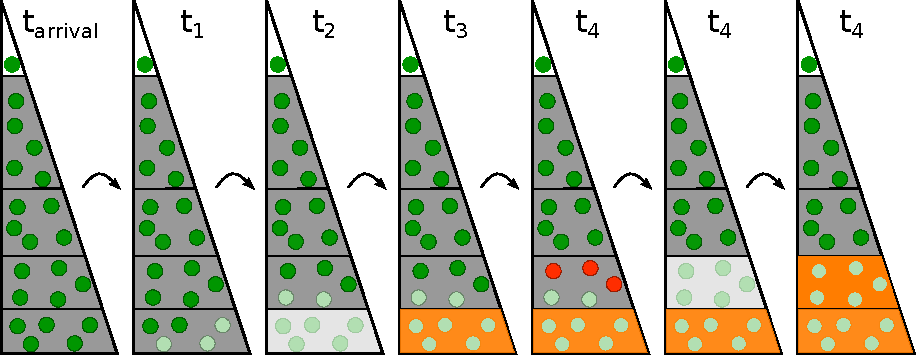
\includegraphics[width=\textwidth]{images/SketchABM2/burningSketch_triangle.pdf}
	\caption{Example of deforestation (by arbitrary agents) in a cell $c$ (black triangle) with an area of $4.2\, \rm{acres}$.
		The cell is arable, with $F_{\rm PI}(c)>0$ and, thus, provides $A_{\rm acres}=4$ farming sites for potential farming (grey areas).
		Initially at $t_{\rm arrival}$, the cell has $21$ trees (carrying capacity).
		At some time $t_{\rm 1}$, after deforestation $18$ of these trees still exist. 
		An Agent $a$ cuts $4$ more trees in the cell (\ra $t_{\rm 2}$). 
		Subsequently, Agent $b$ occupies the cleared site ($1\, {\rm acre}$, light grey area) for farming (orange area) (\ra $t_{\rm 3}$). 
		Finally, an agent $c$, needs to clear $3$ trees by burning them (red dots) to occupy a second site on this cell to fill its farming requirement (\ra $t_{\rm 4}$).}
	\label{fig:treeburning}
\end{figure}

\paragraph{Farming.}
An agent occupies arable land unit sites, $A_\text{F, i}(t)$, with a fixed area of $1\, \text{acre}$ associated to one cell and obtains a yearly farming produce of
\begin{equation}\label{AProd}
F_\text{i}(t) = \sum_{a \, \in \, A_\text{F, i}(t)} \, F_{PI}(c(a))\ ,
\end{equation}
where $a$ denotes a farmed site of $1\, {\rm acre}$ and $c(a)$ is the corresponding cell of this farming site\footnote{Note, for fishers $F_\text{i}(t) = F_\text{Req, i}(t)$ holds immediately without farming and occupying sites.}.
Agents keep all their currently occupied sites $A_\text{F, i}(t)$ until the next year. %, i.e.\ $acres_{\rm i}(t+1) = acres_{\rm i}(t) + new\_acres(t+1)$.
If, over time, an agent $i$'s farming requirement, $F_\text{Req, i}(t)$, increases e.g.\ due to population growth, decrease of the tree preference or erosion of the soil of one of its occupied sites, and consequently the farming produce of the previous year would be insufficient, then the agent needs to occupy more arable sites, i.e.: 
\begin{equation}
F_\text{i}(t-1) < F_\text{Req, i}(t) \ \Rightarrow \ \text{Extend } A_\text{F, i}(t) \text{ and, thus, } F_\text{i}(t) \ .
\end{equation}
%Then the agent occupies more sites extending $A_\text{F, i}(t)$ and, thus, increasing the produce $F_\text{i}(t)$ accordingly.
In the search for new farming sites, an agent first considers only sites in well-suited cells, i.e.\ $c \in C_\text{F}(c_\text{i}(t))$ with $F_\text{PI}(c)=F_\text{PI}|_\text{well}$, in order to maximise farming efficiency.
A site in an arable cell can only be occupied (or added to $A_\text{F, i}(t)$) if at least the corresponding area of $1\, {\rm acre}$ is cleared off trees and not already occupied. 
Assuming that the trees are evenly distributed on the cell's area, the condition can be calculated as 
\begin{eqnarray}
%& \text{Treeless Area\,[acre]} - \text{Occupied Acres\,[acre]}  & \geq 1  \\
%\Leftrightarrow & 
\left( 1 - \frac{T(c,t)}{T(c,t_{\rm arrival})} \right) \cdot A(c) - A_\text{F}(c, t) & \geq   1
\label{eq:BurningCond}
\end{eqnarray}
where the first term is the treeless area in ${\rm acres}$ and the second term, $A_\text{F}(c, t)$, is the number of already farmed sites (by any agent) in cell $c$.%(equation~\ref{eq:occupied}).

If there are no well-suited sites left that fulfil this condition, the agent uses the slash and burn method to remove trees in a well-suited cell $c$ (with at least one unoccupied site).
The agent starts burning trees on the cell that requires the least amount of trees removed for the condition to hold (without leading to soil erosion of the cell, i.e.\ $T(c,t)=0$).
Burning trees and occupying sites continues until the farming requirement of the agent is satisfied or no more well-suited sites are available (even if this leads to soil erosion of the cell).
The use of fires to clear space is supported by the extensive charcoal record starting with the period of intensified agriculture \citep{Mieth2015}. 
Here, I assume that if space is required for farming at time $t$, 
trees are directly burned without being used for any other requirement (assuming this is a more gradual process over the year than the instantaneous burning).
%felled and used (e.g.\ for extraction of the sugar sap) before burning and consequent agricultural use of the land \citep{Mieth2015} or slash and burn method was used directly to clear space as necessary next to tree harvest %(e.g.\ indicated by \citet{Bahn2017}). % Bahn: ``fires directly accompanied by agriculture''
If, all well-suited sites within $C_{\rm F}(c_{\rm i}(t))$ are occupied, but the agent's farming production does not yet meet the requirement ($F_\text{i}(t)<F_\text{Req, i}(t)$), the agent also occupies sites on eroded cells and then on poorly suited cells in the same procedure.

\paragraph{Tree Harvest.}
After fulfilling the farming requirement, the agent cuts down trees according to its tree requirement $T_\text{Req, i}(t)$.
An agent $i$ selects random cells $c\in C_{\rm T}(c_{\rm i}(t))$ with uniform probability and successively removes trees from these cells until the number of cut trees, $T_\text{i}(t)$ matches the requirement $T_\text{Req, i}(t)$ or no further trees are present in $ C_{\rm T}(c_{\rm i}(t))$. 
Unlike farming, where occupied sites are kept and re-used (with the same productivity index) in the next year, the agent obviously needs to find new trees every year.
%Therefore, if tree regrowth is disabled, this tree harvest represents a non-renewable resource dependency of the Easter Island society.
While the agent's adapt their harvest behaviour via the tree preference as this non-renewable resource is depleted over time, a minimum amount of trees is always required and, hence, there's no equilibrium existence of human population without tree regrowth.

\paragraph{Happiness Index.}
A characteristic of the agent is happiness, $h_{\rm i}(t)$, which reflects the success of the harvest of trees and farming production each year.
Here, an agent $i$'s happiness $h_\text{i}(t)$ depends on the ratios of the cut trees, $T_\text{i}(t)$, and farming production, $F_\text{i}(t)$, w.r.t.\ the annual requirements determined beforehand, $T_\text{Req, i}(t)$ and $F_\text{Req, i}(t)$, respectively.
%Assuming that both requirements determine  the tree requirement and the agriculture requirement is equally important to the agent, the happiness is simply the minimum of the fraction of requirements that could be filled:
By assuming that both resources are equally indispensable for the agent, happiness is equal to the smaller of the two fractions:
\begin{equation} 
h_\text{i}(t) = {\rm min} \left( \frac{T_\text{i}(t)}{T_\text{Req, i}(t)}, \, \frac{F_\text{i}(t)}{F_\text{Req, i}(t)} \right)
\label{eq:h_i}
\end{equation}
This is also known as Liebig's law of the minimum, which states that growth is determined by the most scarce resource\footnote{Or: `A chain is only as strong as the weakest link'.}.
If both requirements are filled for agent $i$, the happiness is maximal,  $h_\text{i}(t)=1$.
However, if either $T_\text{i}(t)=0$ or $F_\text{i}(t)=0$, $h_\text{i}(t)=0$ follows regardless of the success in harvesting the other resource.
I assume that households have some resilience to a decline in harvest success (e.g.\ by storing food in more successful years), and, hence, define an effective happiness $H_\text{i}(t)$ as
\begin{equation}
H_\text{i}(t) = \begin{cases} 
				h_\text{i}(t) & \text{ if } h_\text{i}(t)\geq h_\text{i}(t-1) \\
				\frac{h_\text{i}(t) + h_\text{i}(t-1)}{2} & \text{ if } h_\text{i}(t)<h_\text{i}(t-1) 
		\end{cases}
\end{equation}
If an agent's current harvest success decreases (due to resource scarcity), its effective happiness, $H_{\rm i}(t)$, decreases monotonically.
If e.g.\ all trees were to suddenly vanish within a year, an agent would have two years before its effective happiness reaches its minimum $H_\text{i}(t) = 0$.
However, if harvest success increases (e.g.\ due to moving the settlement to a better location), the effective happiness takes on the current happiness value immediately.
As an indicator for successful resource acquisition, the effective happiness $H_\text{i}(t)$ determines the possible responses of agent $i$ to the harvest, which I describe in Sections \ref{sec:PopGrowth} and \ref{sec:Moving}.

%\footnotetext{One could also frame this as a discounting factor. If resources are scarce, }

%\section{Responses of Agent Features Following the Resource Acquisition}\label{sec:Reaction} 
\FloatBarrier
\section{Population Growth}\label{sec:PopGrowth}
\paragraph{Stochastic, Discrete Population Growth.}
Following the interaction between the agent and the environment through farming and tree cutting, the agent's population size $pop_{\rm i}(t)$ adapts. 
The net (positive or negative) growth rate of the agent's population at a specific time depends only on the effective happiness and, thus, harvest success:
\begin{equation}\label{eq:popgrowthcontinuos}
pop_{\rm i}(t+1) = (1+g(H_{\rm i}(t))) \cdot pop_{\rm i}(t)
\end{equation}
In fact, instead of assuming continuous growth or decline according to this growth rate, $g(H_{\rm i}(t))$, the population dynamics is implemented as a discrete, stochastic process.
Each individual of the household agent has a $|g(H_{\rm i}(t))|$ probability to die if $g(H_{\rm i}(t))<0$, or %a $g(H_{\rm i}(t))-1$ chance 
to reproduce (i.e.\ adding one individual to the household/agent) if $g(H_{\rm i}(t))>0$.
The population size stays constant at $H_{\rm i}(t) = H_{\rm equ}$ with $g(H_{\rm equ}(t))=0$. 
This results in a stepwise growth/decline of the population in which each agent's population size trajectory is a single realisation of the stochastic process which on average matches the continuous dynamics in equation~\ref{eq:popgrowthcontinuos} (compare e.g.\ with \citen{Bungartz2009}).
Note, $g(H_{\rm i}(t))$ represents a harvest dependent stochastic, discrete \textit{excess} growth or decline rate. 
I assume that `base' (i.e.\ for $H_{\rm i}(t) = H_{\rm equ}$ and, thus, $g(H_{\rm equ})=0$) deaths and births average out for each year in spite of the fact that this too is a stochastic discrete process \citep{Bungartz2009}.
Figure \ref{fig:realisationsofpopgrowth} in the Appendix shows a few different realisations of a discrete, constant (excess) growth scenario with rate $g(H_{\rm i}(t)=1)=0.7\%$ (i.e.\ with unlimited resource availability) in comparison to continuous growth.

\paragraph{Growth with Unlimited Resources.}
There is a strong debate about the initial growth rate of the Easter Island population after the arrival of a small number of Polynesians.
This corresponds to the growth rate, $g(H_{\rm i}(t))$, without resource constraints and, thus, $H_{\rm i}(t)=1$.
Parameters found in the literature range from $0.7\%$ per year \citep{Bahn2017} or `always below $1\%$' \citep{Brander1998} to more than $3\%$ \citep{Hunt2007} for short periods of time or $2.3-4.5\%$ \citep{Brandt2015}.
Depending on the proposed chronology, researchers have to make very contrary assumptions on population growth in order to fit the population dynamics to the few undisputed facts about the historic Easter Island civilisation. 
If an arrival around $1200\, \text{A.D.}$ is assumed (as in \citen{Hunt2007}, or \citen{Brandt2015}), a large population growth is unavoidable\footnote{E.g.\ as it seems impossible that only a few hundred inhabitants in the 13th to 16th century could have created several hundred Moai statues (and caused a massive alteration of the island's environment)}.
Slower initial population growth needs to be assumed in studies proposing earlier arrival dates (around $800\, \text{A.D.}$ e.g.\ in \citen{Bahn2017}), or even as early as $400\, \text{A.D.}$ in \citen{Good2006}, and \citen{Brander1998})\footnote{given that archaeological data indicates an intensification of human activity, which suggests a large population size, only starting after $1200\, \text{A.D.}$ (e.g.\ \citen{Bahn2017} and \citen{Hunt2007}).}.
Other hypothesis, such as multiple, distinct periods of population growth and declines have been put forward (e.g.\ \citen{Cole2008}), but do not seem to be common in the context of Easter Island.
Following the traditional hypothesis of an early arrival, e.g.\ in \citet{Bahn2017}, I choose an $t_\text{arrival}=800\, A.D.$, as described before, and, thus, a slow growth rate (in one year) in the case of unlimited resource access and, therefore, continuously happy agents: 
\begin{equation}
	g(H_\text{i}(t)=1) = 0.7\% \ .
\end{equation}

\paragraph{Growth or Decrease with Limited Resources.}
The dependency of the population growth or decline rate, $g(H_{\rm i}(t))$, in the case of limited resources, i.e.\ $H_{\rm i}(t)<1$, is a further uncertainty in modelling human-resource interactions in general.
\citet{Lee2008} and \citet{Puleston2008} constructed a food-limited demography model, which was later applied to Easter Island \citep{Puleston2017}. 
Here I use a strongly simplified assumption of this model to parametrise the impact of non-optimal harvests on the population dynamics. 
The authors derived age-dependent survival and fertility rates, which are both S-shaped curves w.r.t.\ food availability (i.e.\ high in the case of unlimited food availability and low in the case of scarce food availability).
Since I do not consider age structures, I simply assume a net growth rate with the same shape as the survival and fertility rates in \citet{Lee2008}.
\begin{equation}
g(H_\text{i}(t)) \sim \text{CDF}(\Gamma_\text{Dist}(shape, scale=0.1))
\end{equation}
where $\text{CDF}(\Gamma_\text{Dist})$ is the cumulative density function of the Gamma distribution (characterised by shape and scale parameter) with scale fixed as in \citet{Lee2008}.
I then tune the shape parameter of this function to obtain the same equilibrium point $g(H_\text{i}(t) =H_\text{equ})=0$ as \citet{Puleston2017}, at which the population size remains constant:
\begin{equation}
H_\text{equ}=0.6883 \quad \text{with } g(H_\text{i}(t) = H_\text{equ})=0   \ .
\end{equation} 
This corresponds to $shape=1.95$, which I use in the standard configuration.
In order to test sensitivity of the results w.r.t.\ this parameter choice, I also investigate a larger shape parameter $shape^*=3$ with $H_{\rm equ}^*=0.84$, which leads to a less resilient population size when resource scarcity sets in.
The amplitude of the resulting function (for both scenarios) is scaled to give the chosen reproduction rate under unconstrained food supply from last paragraph 
$g(H_\text{i}(t)=1)=0.7\%$.
Figure \ref{fig:growthrate} shows the results of this dependency (standard setting in blue and less resilient setting in red) with the happiness regime for net growth, $H_\text{i}(t) > H_{\text equ}$ (with a maximum of $g(H_\text{i}(t)=1)=0.7\%$) and the regime for net decline of the population size, $H_\text{i}(t) < H_{\text equ}$.
\begin{figure}
	\centering
	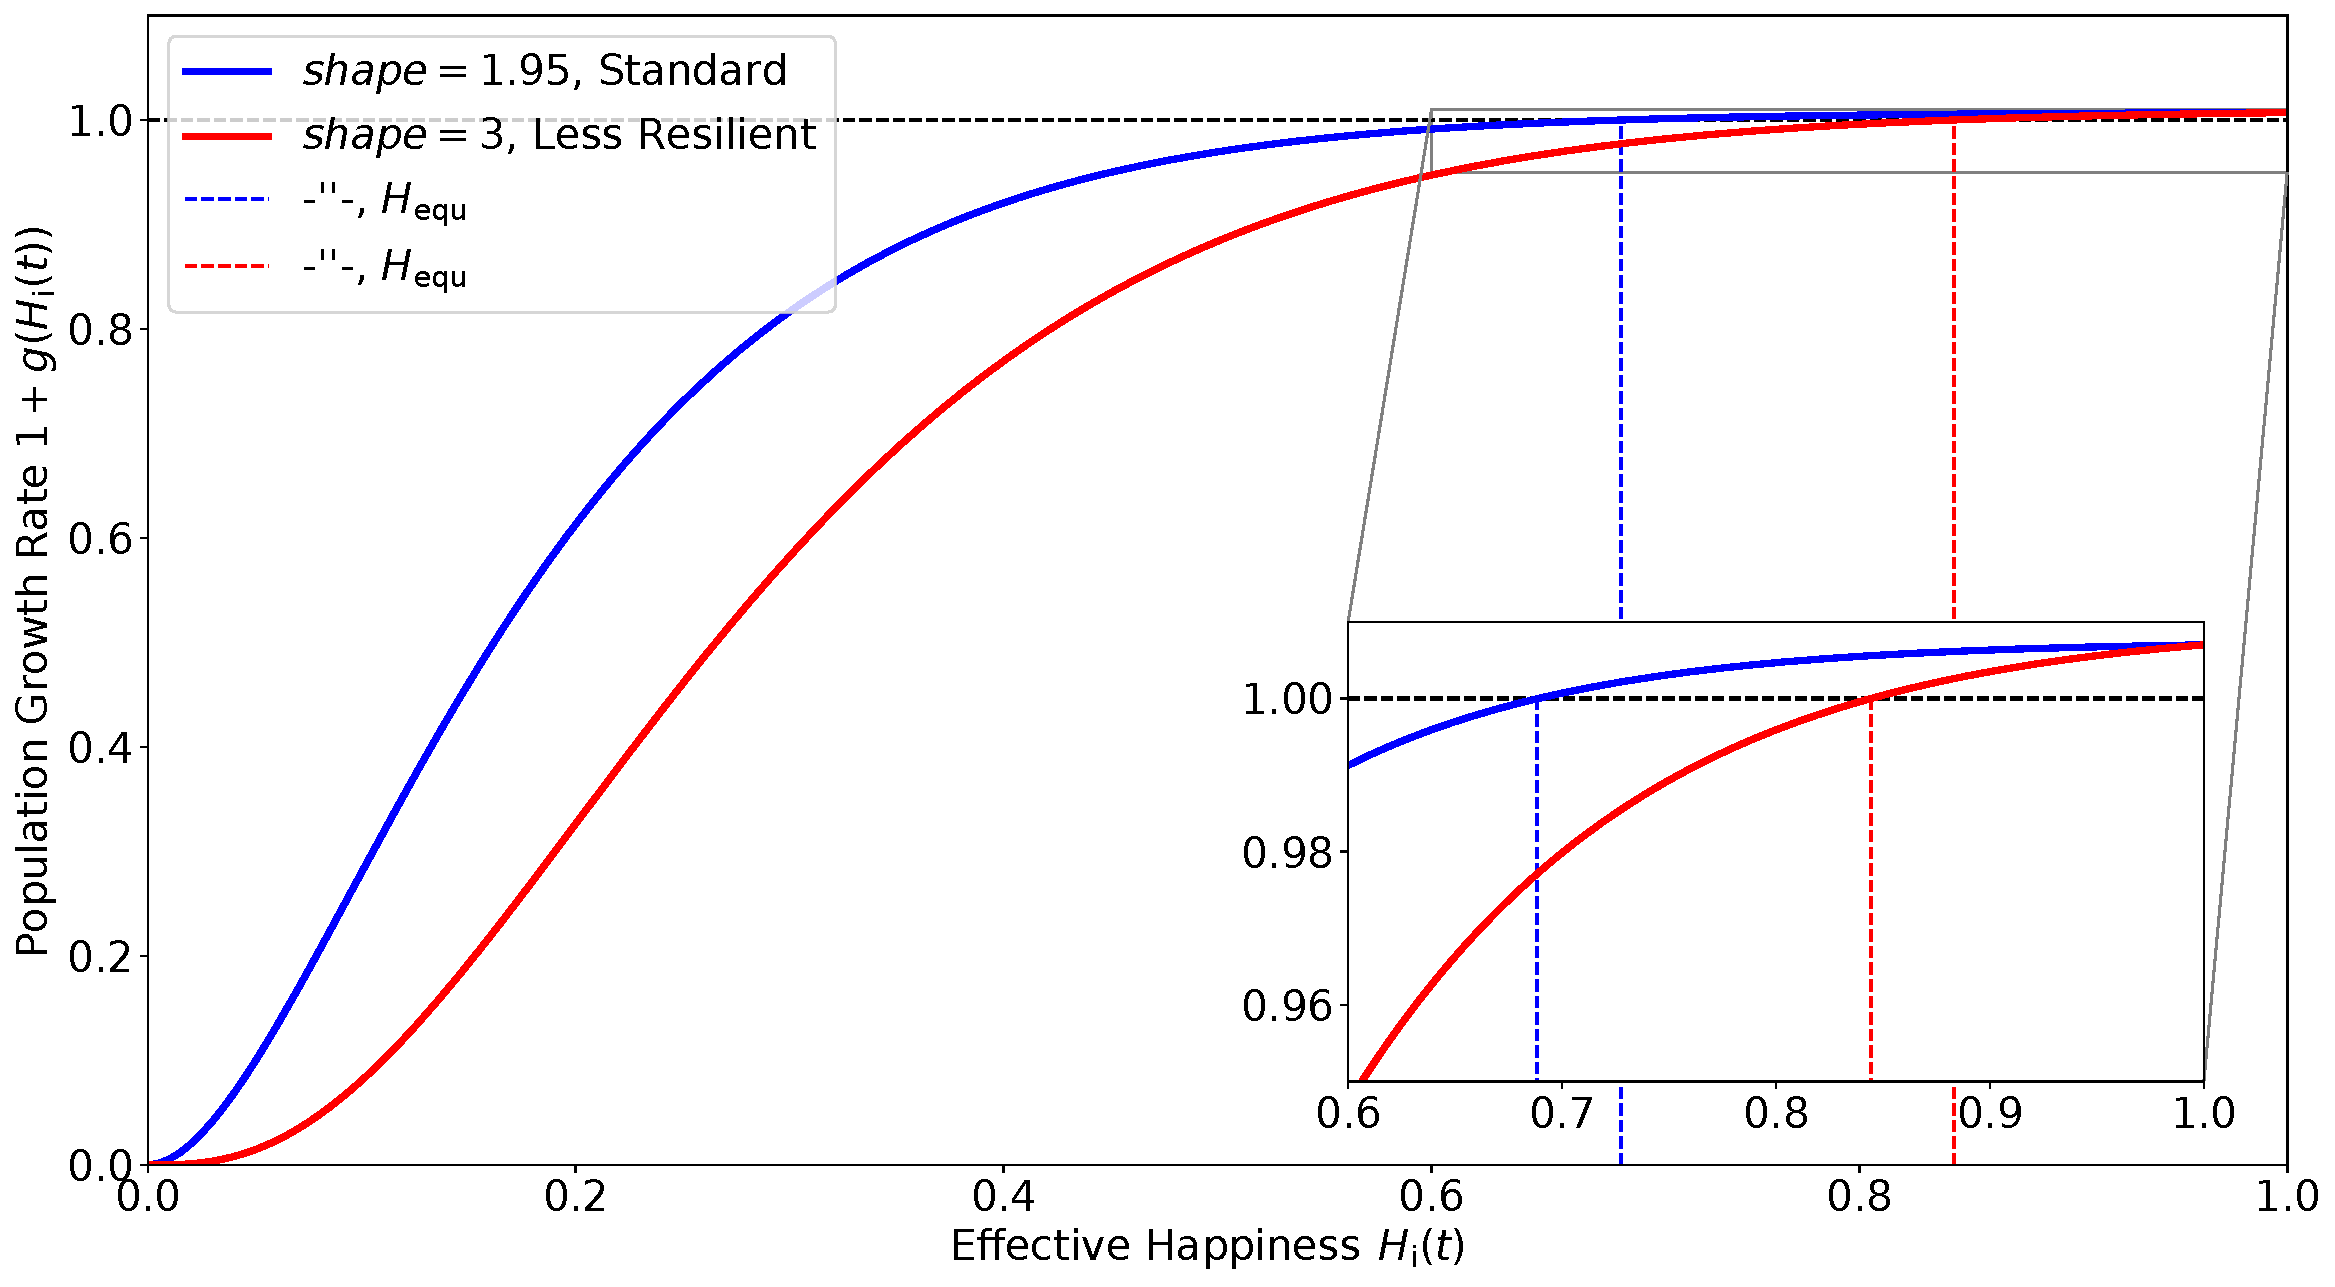
\includegraphics[width=\textwidth]{images/populationchange_g}
	\caption{The growth rate of an agent's population size as a function of its effective happiness $H_{\rm i}(t)$. Functional dependence follows simplified assumptions made in the food-limited demography model by \citet{Lee2008}, \citet{Puleston2008}, and \citet{Puleston2017}. In the standard scenario (red) the agent's population size grows if $H_{\rm i}(t)>H_{\rm equ}=0.6883$ and declines for smaller $H_{\rm i}(t)$. An alternative, less resilient scenario is also tested, with a smaller population growth regime of $H_{\rm i}(t)>0.84$. The maximum growth rate in the case of maximum happiness (and thus unconstrained resource availability) is $g(H_{\rm i}(t)=1)=0.7\%$.}
	\label{fig:growthrate}
\end{figure}

% Topic SPLITTING THE AGENT
\paragraph{Splitting or Removal of an Agent.}
There are upper and lower limits to the population size of an agent, causing it to split or disperse.
If the population size $pop_{\rm i}$ of an agent $i$ falls below a certain threshold $pop_{\rm min} = 6$, the agent $i$ is removed and the remaining individuals are adopted by other households chosen randomly within the moving radius distance, $r_{\rm M}$ ($C_{\rm M}(c_{\rm i})$ defined later).
If the household's population becomes too large, a subgroup splits from it forming a new agent.
According to \citet{Bahn2017}, settlements found in archaeological excavations consisted of two to three dwellings, the basic domestic units (e.g.\ caves or stone houses). 
Assuming that roughly a dozen people can live in such a dwelling, which would include the larger family, a household includes around $30$ ($2.5\cdot 12$) individuals.
In this model, if the population size reaches values requiring more than three dwellings, a dozen individuals split off and start a new settlement in a different location on the island. 
The stochastic splitting probability given an agent's population size is
\begin{equation}
Pr_{\rm splitting} = \mathcal{N}( \mu = pop_\text{split, mean}, \sigma = pop_\text{split, std})\ ,
\end{equation}
i.e.\ a Gaussian distribution with mean $pop_\text{split, mean} = 3.5 \cdot 12 = 42$ and standard deviation $pop_\text{split, std} = 3$.
The remaining household with reduced population size and, thus, smaller farming requirement then frees up no longer required sites for farming\footnote{Sites with lower farming productivity first.}.
The splitting agent, immediately moves to a new location determined by the moving process described in Section~\ref{sec:Moving}.
In summary, an agent represents a household of typically $12$ (with a lower limit of $6$) to ca.\ $42\pm 3$ individuals. % that acts independent of other agents.

\FloatBarrier
\section{Movement of Agents}\label{sec:Moving}
% When to move
\paragraph{Procedure and Condition for Moving.}
Agents relocate their settlement either in response to insufficient harvest or after splitting from a large household to start a new settlement.
An agent abandons the settlement if, after the harvest, its smoothed happiness is below the equilibrium point $H_\text{equ}=0.6883$ (in the standard setting), i.e.\ net negative population growth $g(H_\text{i}(t))\leq 0$.
The agent first chooses a cell within a certain radius according to probabilities that reflect how high the agent evaluates this location based on several different categories.
Within this new cell, the agent chooses a location according to a uniform probability and settles there.

% How to calculate moving radius
\paragraph{Moving Radius.}
In the initial phase of the simulation, agents can choose new locations from all cells on the island\footnote{Except for the initial settlers who are assumed to settle close to the landing spot, Anakena Beach}.
However, if a certain total population size is exceeded (here $\mathbf{pop}(t)\geq \mathbf{pop}_\text{restricted moving} = 5000 \, \rm{people}$), a restriction of the agents' ability to move around freely is enforced and, therefore, new settlements are only allowed within a certain radius of the agent's old location.
When relocating the settlement, an agent $i$, thus, chooses from cells:
%Thus, the cells considered as potential new location for an agent $i$ are
\begin{equation}
C_{M}(c_{\rm i}, \mathbf{pop}(t)) = 
\begin{cases}
\{\tilde{c} \ | \ \tilde{c}\text{ on island}\} & \text{ if } \mathbf{pop}(t) <5000 \\
\{\tilde{c} \ | \ | | \vec{\tilde{c}} - \vec{x_{\rm i}}(t) | |
%\begin{pmatrix} \tilde{c}_x \\ \tilde{c}_y \end{pmatrix}  - \begin{pmatrix}x_i\\ y_i \end{pmatrix} 
\leq r_{\rm M} \} & \text{else} 
\end{cases}
\end{equation}
with radius $r_{\rm M} = 5\, {\rm km}$.

% Topic: It's a decision making process.
%Determining the new location for an agent represents a decision-making process through evaluation of sites by the agent.
\paragraph{Deciding on the New Location.}
In a semi-rationale decision making process the agents choose a new location by evaluating cells $c$ within $C_{\rm M} (c_{\rm i}, \mathbf{pop}(t))$ according to probabilities inferred from several different penalties:
%The calculation of the probability to move to a specific cell bases on penalties from the following categories: 
$P_{\rm G(c)}$ for geographical constraints, $P_{\rm W}(c)$ for distance from freshwater, $P_{\rm D}(c)$ for population density, $P_{\rm T}(c)$ for tree availability, and $P_{\rm F}(c)$ for farming land availability.
High penalties represent unfavourable conditions (in the specific category) for settling in the specific cell.


%TOPIC: LOGISITIC FUNCTIONS
\paragraph{General Calculation of Penalties.}
Penalties for each category $P_{\rm X}$ ($X=\{\text{G,\, W, \, D,\, T,\, F}\}$) are calculated with logistic functions depending on one characteristic evaluation variable $x$ ranging from $x_{\rm min}$ to $x_{\rm max}$.
In reality such an evaluation would typically depend on more than one variable and might be related to complex functional behaviour.
However, the assumption made here is a plausible simplification given that with the logistic function there is a range of values of the evaluation variable indicating favourable conditions (with negligible penalties) and a range of values indicating unfavourable conditions (with high penalties)\footnote{For example an agent might assign the same penalty to two locations $100\, \text{m}$ and $500\, \text{m}$ away from a large freshwater source. If instead the nearest lake is too far away from the agent to rely on it for everyday use, alternative sources have to be found, regardless of whether the distance is $5$ or $10\, {\rm km}$ and therefore, the penalty is similarly high.}.
I determine the shape of the function of $P_X$ of variable $x$ through `thresholds' $x_{\rm P0.01}$ and $x_{\rm P0.99}$ indicating the value of $x$ at which the penalty $P_{\rm X}$ is smaller than $1\%$ (favourable conditions) or larger than $99\%$ (unfavourable conditions), respectively, in this category $X$.
The penalty $P_{\rm X}$ in a cell $c$ with value $x(c)$ is then
\begin{eqnarray}\label{eq:P_X(c)}
	P_{\rm X}(c) & = & \frac{1}{1+\exp\left( - k_{\rm X} (x(c)-\frac{x_{\rm P0.01}+x_{\rm P0.99}}{2}) \right)} %= \\
%		& = & \begin{cases}
%	<0.01  & \text{ for }x_{\rm min}<x(c)<x_{P0.01} \\
%	\text{?}  & \text{ for } x_{P0.01}\leq x(c) \leq x_{P0.99} \\
%	>0.99  & \text{ for }x_{P0.99}<x(c) < x_{\rm max} \\	
%	\end{cases}
\end{eqnarray}
where steepness $k_{\rm X}$ is 
\begin{equation}\label{eq:k}
k_{\rm X} = \left(\frac{x_{\rm P0.99}-{x_{\rm P0.01}}}{2}\right)^{-1} \cdot \log\left(\frac{0.99}{0.01}\right) \ .
\end{equation}
to fix the penalty to the respective values at thresholds $x_{\rm P0.01}$ and $x_{\rm P0.99}$.
This function is shown for a general case in Figure \ref{fig:logF}.
\begin{figure}
	\centering
	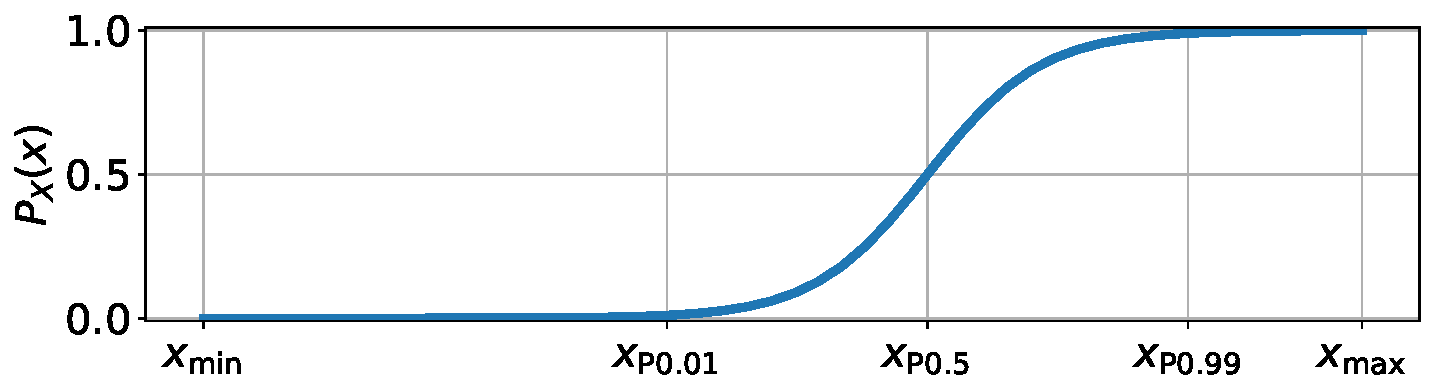
\includegraphics[width=\textwidth]{images/general_logF.pdf}
	\caption{General shape of the logistic function $P_{\rm X}(c)$ for a penalty for moving to a certain cell $c$ in the category $X$ ($\in\{\text{W, G, D, T, F}\}$). The penalty depends on a characteristic variable $x$, in combination with the thresholds, $x_{\rm P0.01}$ and $x_{\rm P0.99}$ (and $x_{\rm min}$ and $x_{\rm max}$) and, thus, the steepness parameter $k_{\rm x}$.}
	\label{fig:logF}
\end{figure}
For each category $X$, this logistic function has the same (relative) shape between $x_{\rm P0.01}$ and $x_{\rm P0.99}$. % given by $k_{\rm x}$. 
Hence, the sensitivity of penalty $P_{\rm X}$ to differences in variable $x$ is determined from $x_{\rm P0.01}$ and $x_{\rm P0.99}$, and thus, $k_{\rm x}$.
If the values of $x_{\rm P0.01}$ and $x_{\rm P0.99}$ are close, equation \ref{eq:P_X(c)} converges to a sigmoid function. 
If they are far apart, the function resembles a less steep increase of the penalty $P_{\rm X}$ with $x$.
For $x=\frac{x_{\rm P0.01} + x_{\rm P0.99}}{2}$ the penalty is $P_{\rm X} = 50\%$.
Note, that if $x$ is chosen such that large values are favourable (e.g.\ for the tree and farming penalty), choosing values $x_{\rm P0.01}>x_{\rm P0.99}$ simply mirrors the logistic function in equation \ref{eq:P_X(c)} at its midpoint $x=\frac{x_{\rm P0.01}+x_{\rm P0.99}}{2}$. %and all `$<$' or `$>$' signs accordingly.
In summary, this logistic dependence of penalties on characteristic variables represents a non-linear evaluation of locations.

%The steepness $k_0$ can be chosen, such that the different cases of function $P_X(x)$ are reasonably close at the threshold values $x_{\rm P0.01/P0.99}$. 
%Here, I choose $k_0 = \left( \frac{x_{\rm P0.01}-{x_{\rm P0.99}}}{2}\right)^{-1}\cdot \log\left(\frac{0.01}{0.99}\right)$, giving $P_{\rm X(x=x_{\rm P0.01})=0.01$ and $P_{\rm X(x=x_{\rm P0.99}) = 0.99$.
%Higher $k_0$ results in a steeper increase of the penalty with $x$.
%Nevertheless, this choice for parametrising a complex decision making process as well as the values for the thresholds are very flexible. 
%Of course, we can not know how Easter Island households evaluated potential new settlement areas.
%Nevertheless, archaeological data as well as logic surely show that the island has been settled progressively, e.g.\ \citet{Bahn2017}. Hence, it can be very useful to understand what 
%However, it reflects a decision. 

% Following up: Penalty Categories and summary in sketch and table
%The parametrisation of evaluating new locations is, of course, strongly simplified. 
%First, the decision making typically depends on more than one evaluation variable per penalty category, as assumed here.
%Secondly, the functional dependency of penalty w.r.t.\ the evaluation variable in general is more complex than the simple logistic evaluation in equation~\ref{eq:P_X(c)}.
%However, assuming that advantages and disadvantages of a potential location (summarised in a single variable) play a non-linear role in the agent's decision making, the use of a logistic function seems reasonable\footnote{For example an agent might assign the same penalty to two locations $100\, \text{m}$ and $500\, \text{m}$ away from a large freshwater source. 
%If instead the nearest lake is too far away from the agent to rely on it for everyday use, alternative sources have to be found, regardless of whether the distance is $5$ or $10\, {\rm km}$ and therefore, the penalty is similarly high.}.

\paragraph{Parameter Choices.} %for $\mathbf{P_{\rm X}(x)}$}
I determine the choice of the evaluation variable $x$ and thresholds $x_{\rm P0.01}$ and $x_{\rm P0.99}$ via plausible, heuristic arguments or estimates.
The following paragraphs point out the motivation for the specific variables for the agent's evaluation process and the threshold choices in the standard configuration of the model for each penalty category $P_{\rm X}$ ($X=\{\text{G,\, W, \, D,\, T,\, F}\}$).
Table \ref{tab:x01x09} summarises the variables and corresponding thresholds that together with equation~\ref{eq:P_X(c)} determine the penalties $P_{\rm X}$ w.r.t.\ $x$ for all categories and thus the decision making of an agent when relocating the settlement.
%All of these contributions in a cell $c$ are then linearly combined to a total penalty for this cell $P_{tot}(c)$. 

%\begin{figure}
%	Logistic Functions
%	\label{fig:Logistic}
%\end{figure}

% TOPIC: Water Distance PEnalty
\paragraph{Distance from Freshwater.}
There are very limited permanent sources of freshwater on the island, making it an important factor of settlement behaviour. 
Nearly all studies on Easter Island history point out that the lakes inside the three volcano craters (Rano Kau in the South, Rano Rarakua in the East, and Rano Aroi in the North, cf.\ Figure \ref{fig:Karte}) are the main freshwater reservoirs\footnote{Other potential sources include pools in lava tubes and springs in the North Coast (all mentioned in \citen{Bahn2017}), an intermittent stream from Mount Terevaka, wells and water bubbles at low tide, and sugar cane juice (all mentioned in \citen{Diamond2011}), 
Additionally, \citet{Mieth2015} emphasizes the possibility to obtain a sugary sap from cut palm tree trunks, which could have replaced the need for freshwater for a large share of the population.
However, crater lakes are the most reliable (and accessible) large freshwater supply.}
and, thus, are `obvious centres for human activity' \citep{Bahn2017}.
%Topic Variable xC
Consequently, I assume that potential locations close to (large) lakes are more likely settled.
The evaluation variable $w$ radially increases with the distance to the nearest lake weighted by the lake area:
\begin{equation}
	w = min_{\text{lake}\in \text{[Kau, Raraku, Aroi]}} \left( \frac{||
		%\begin{pmatrix} c_x \\ c_y \end{pmatrix}  - \begin{pmatrix} \vec{lake}\\ y_i \end{pmatrix}
		 \vec{c}- \vec{lake}||^2}{r_\text{lake}^2\pi} \right)
\end{equation}
%\begin{equation}
%	P_W(c) = \frac{1}{N} \cdot min_{\text{lake}\in \text{[Kau, Raraku, Aroi]}} \left( \frac{\text{dist(lake, c)}^2}{r_\text{lake}^2\pi} \right)
%\end{equation}
with estimated radii of the lakes $r_\text{Kau} = 506\, \rm{m}$, $r_\text{Raraku} = 170\, \rm{m}$, $r_\text{Aroi} = 75\, \rm{m}$ and $\vec{lake}$ representing the position of the cells corresponding to the lakes.
%Here, $dist$ is the minimum straight line distance between a lake and the cell's midpoint.
%$N$ is a normalisation factor, such that the penalty $P_{\rm W}\in[0,1]$.
The thresholds are chosen as 
\begin{equation}
w_{\rm P0.01} = \frac{(0.5\, {\rm km})^2}{r_\text{Raraku}^2\pi} \qquad
 w_{\rm P0.99}=\frac{(5\, {\rm km})^2}{r_\text{Raraku}^2\pi}
\end{equation} 
($0.5$ and $5\, {\rm km}$ distance of a lake like Rano Raraku, respectively).
Then, $P_{\rm W}(c)$ is calculated from equation \ref{eq:P_X(c)} with evaluation variable $w$, the corresponding thresholds and $k_{\rm W}$ as in equation \ref{eq:k}:
\begin{equation}
	P_{\rm W}(c) = \frac{1}{1+\exp\left( - k_{\rm W} (w(c)-\frac{w_{\rm P0.01}+w_{\rm P0.99}}{2}) \right)} \ .
\end{equation}
Drought periods during the Medieval Climate Anomaly (period before $1200\, {\rm A.D.}$) and the Little Ice Age ($1570-1720 \, {\rm A.D.}$) potentially led to a dessication of Rano Raraku \citep{Rull2020}, which is also incorporated here by simply removing the lake in the corresponding years from the discretised map. 
%Hence, during drought periods the locations around Rano Raraku have a substantially higher water penalty $P_{\rm W}$.
%The penalty is cut-off at its maximum value $1$, even for this case with higher penalties.
%Except for these droughts, the water penalty is constant for all agents and times.
A map of the constant $P_{\rm W}(c)$ (without drought) is shown in Figure \ref{fig:plotpw}. 
\begin{figure}
	\centering
	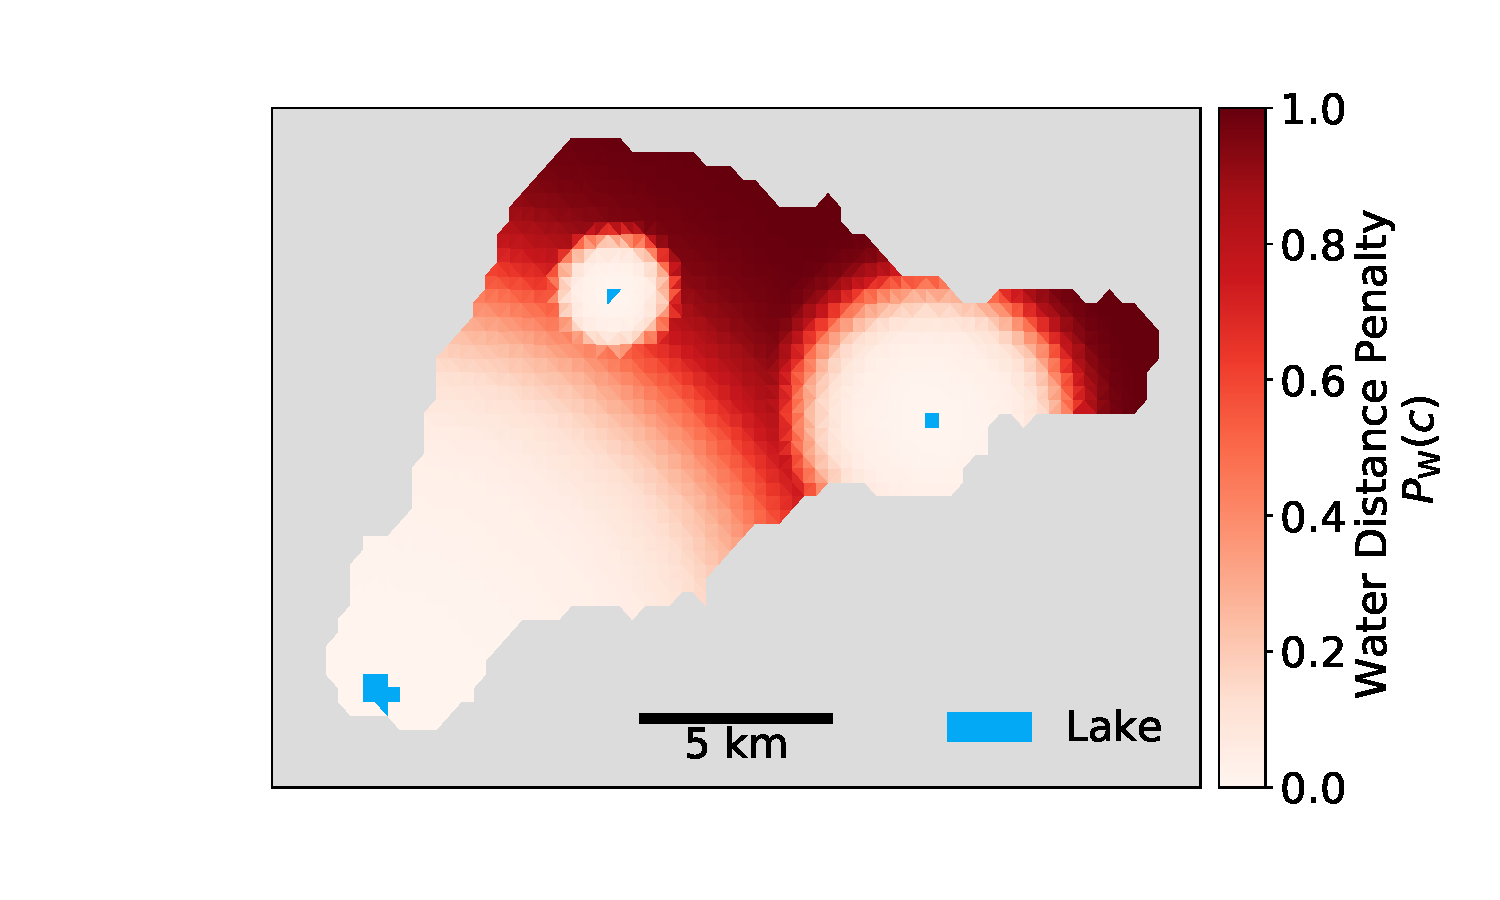
\includegraphics[width=1\linewidth]{images/Plot_PW}
	\caption{The water penalty $P_{\rm W}(c)$ for all cells in times without drought, i.e.\ when Rano Raraku (in the East) provides freshwater.}
	\label{fig:plotpw}
\end{figure}


%Topic: Elevation Slope
\paragraph{Geographical Constraints.}% $P_{\rm G}$
High elevation and slope of Easter Island further penalise the settlement probabilities in this model.
Archaeological evidence (e.g.\ the distribution of the Ahu and Moai) shows that the first $1-2\, \rm{km}$ inland from the coast were the preferred settlement locations, even if upland locations were farmed \citep{Bahn2017}.
There are several possible reasons for that including easier access to small-scale fishing, climatic conditions, or cultural reasons.
Hence, I assume that the geographical penalty depends on a cell's elevation.
The evaluation variable is $el(c)$ and the chosen thresholds $el_{\rm P0.01}=min_{\rm c}(el(c))=0\, {\rm m}$ and $el_{\rm P0.99}=max_{\rm c}(el(c)) = 300\, {\rm m}$ (arbitrary choice).
Furthermore, the North West coast and the areas around the volcano craters are steep, making it difficult for large households to settle in these spots, e.g.\ due to the danger of land slides. 
Hence, the geographical penalty also depends on a cell's slope.
The evaluation variable is $sl(c)$ and the corresponding chosen thresholds $sl_{\rm P0.01}=0^\circ$ and $sl_{\rm P0.99}=7.5^\circ$ (arbitrary choice). 
Then, with corresponding $k_{\rm el}$ and $k_{\rm sl}$ from equation~\ref{eq:k}, the penalties for terrain elevation and slope are calculated as 
\begin{eqnarray}
	P_{\text{el}}(c) = \frac{1}{1+\exp\left( - k_{\rm el} (el(c)-\frac{el_{\rm P0.01}+el_{\rm P0.99}}{2}) \right)}\\
	P_{\text{sl}}(c) = \frac{1}{1+\exp\left( - k_{\rm sl} (sl(c)-\frac{sl_{\rm P0.01}+sl_{\rm P0.99}}{2}) \right)}
\end{eqnarray}
The (combined) geographical penalty $P_{\rm G}$ for a cell $c$ is simply the average of $P_{\rm el}$ and $P_{\rm sl}$:
\begin{equation}
%P_{\rm G}(c) = \rm{max}\left(P_\text{el}(c), P_\text{sl}(c) \right)
P_{\rm G}(c) = \left(P_\text{el}(c)+P_\text{sl}(c) \right)/2
\end{equation}
Figure \ref{fig:P_G} shows the geographic penalty, $P_{\rm G}$, which is the same for all agents and constant over time.
\begin{figure}
	\centering
	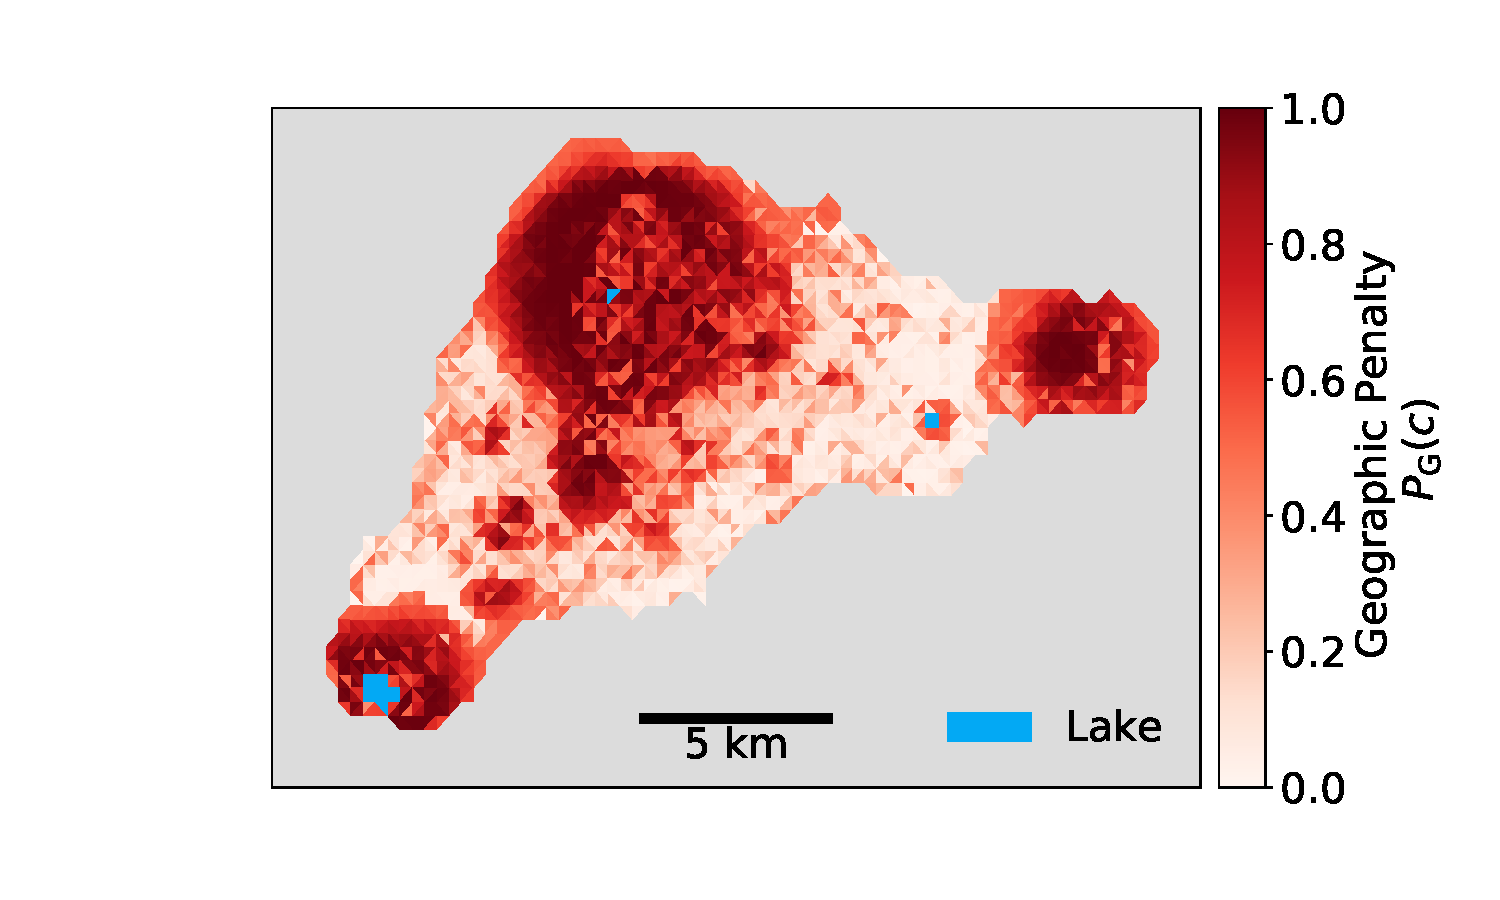
\includegraphics[width=1\linewidth]{images/Plot_PG}
	\caption{The constant geography penalty $P_{\rm G}$ for all cells.}
	\label{fig:P_G}
\end{figure}

% TOPIC: Pop Density Penalty
\paragraph{Population density.} % $P_{\rm D}$
Agents also avoid moving to locations with a large population density.
While different agents share the same resources and, thus, interact with the same environment, their actions and moving decisions are independent from each other. 
However, by making locations with high population density unfavourable, the population penalty introduces an indirect agent-agent interaction. 
%To some degree, this is incorporated in the farming penalty (later) as well, as regions with large population density, also have fewer available agriculture sites.
I define the population density of a cell as the population density within the farming radius of cell $\tilde{c}$, i.e.\ $C_{\rm F}(\tilde{c})$.
\begin{equation}
pd (\tilde{c}) = \frac{\mathbf{pop}|_{\hat{c} \in C_{\rm F}(\tilde{c}) }}{r_{\rm F}^2 \pi}
\end{equation}
The thresholds are chosen as
\begin{equation}
pd_{\rm P0.01} = 0 \, {\rm \frac{ppl}{km^2}}
\end{equation}
and 
\begin{equation}
pd_{\rm P0.99} = 300 \, {\rm \frac{ppl}{km^2}}
\end{equation}
with estimated values of $262$ and $389\, {\rm \frac{ppl}{km^2}}$ on `prime agricultural land' on Hawaii and Maui (\citen{Kirch2010}; \citen{Puleston2017}), which likely overestimate the maximum local densities on Easter Island \citep{Puleston2017}. %Puleston state that!!
%The latter is chosen from local population density estimates of \todo{Puleston 558}.
Then, the (time dependent) population density penalty for one cell is
\begin{equation}
P_{\rm D}(\tilde{c}) = \frac{1}{1+\exp\left( - k_{\rm D} (pd(\tilde{c})-\frac{pd_{\rm P0.01} + pd_{\rm P0.99}}{2}) \right)}
\end{equation}
with the corresponding $k_{\rm D}$ calculated from equation~\ref{eq:k}.
		
% TOPIC: Tree Penalty
\paragraph{Availability of Trees.} %$P_\text{T}$
Scarcity of trees in the local surrounding of a specific location also penalises a possible settlement.
The tree penalty $P_{\rm T}(\tilde{c})$ is determined via the evaluation variable $tr(c)$, the number of trees within $C_{\rm T}(\tilde{c})$,
\begin{equation}
	tr(\hat{c}) = \sum_{\hat{c} \in C_{\rm T}(\tilde{c})}\, T(\tilde{c},t) \ .
\end{equation}
A cell with large value of $tr$ has a lower tree penalty.
There is no intuitive threshold for having a negligible tree penalty, $tr_{\rm P0.01}$ (or optimal number of trees).
Here, I choose this value as the tree number sufficient to fill the tree requirement for a population of very high density, $pd = pd_{\rm P0.99}$, in the tree search radius, $C_{\rm T}(c_{\rm i}(t))$, with maximum tree preference $T_\text{Pref, max}$ for roughly one generation ($\sim 45\, {\rm yrs}$).
\begin{equation}
tr_{\rm P0.01} = T_\text{Pref, max} \cdot T_\text{Requ, pP} \cdot \left(pd_{\rm P0.99} \cdot \frac{r_{\rm T}^2}{r_{\rm F}^{2}}\right) \, {\rm ppl} \cdot 45\, {\rm yrs} = 
216\cdot 10^3 \, {\rm trees} \ .
\end{equation} 
The threshold, $tr_{\rm P0.99}$, is chosen as the tree number required to keep the current agent's population at a happiness level of at least $h_{\rm i}(t) = H_{equ}$ for the next year:
\begin{equation}
tr_{\rm P0.99, i}= T_\text{Pref, i}(t) \cdot T_\text{Req, pP} \cdot pop_{\rm i}(t) \cdot H_\text{equ} \ ,
\end{equation}
which is typically between $10-100\, {\rm trees}$ depending on the properties of agent $i$.
On top of the logistic penalty dependency, I further enforce a necessary condition of tree availability at $tr_{\rm P0.99}$: 
A cell $\tilde{c}$ is only considered as viable settlement location if the number of trees at least fulfils $tr(\tilde{c}) \geq tr_{\rm P0.99}$. 
In total, 
\begin{equation}
P_{\rm T, \ i}(\tilde{c}) = 
\begin{cases} \infty & \text{ if }tr(\tilde{c})< tr_{\rm P0.99} \\
\frac{1}{1+\exp\left( - k_{\rm tr} (tr(\tilde{c})-\frac{tr_{\rm P0.01}+tr_{\rm P0.99}}{2}) \right)} & \text{ else }
\end{cases}
\end{equation}


% TOPIC: Agric Penalty
\paragraph{Availability of Farming Land.}%$P_{\rm F}$
%Location penalised by agriculture
Finally, also availability of farming sites influences the agent's moving decision.
The penalty for farming, here, depends on two evaluation variables: 
The total available farming potential $F_\text{tot}(\tilde{c})$ and the available farming potential from non-eroded, well-suited cells only, $F_\text{well}(\tilde{c})$.
The penalties for both variables are calculated separately and then averaged.
The total available farming potential is simply a summation of all productivity indices of arable, unoccupied sites (number of sites within a cell) within $C_\text{F}(\tilde{c})$.
\begin{equation}
	F_\text{tot}(\tilde{c}) = \sum_{\hat{c} \in C_{\rm F}(\tilde{c}) }\, F_{\rm PI}(\hat{c}) \cdot (A_{\rm acres}(\hat{c})  - A_{\rm F}(\hat{c}, t) ) \ ,
\end{equation}
where $A_{\rm acres}(c)$ is the number of farming sites and $ A_{\rm F}(c,t)$ is again the number of occupied sites (and, therefore, unavailable to new agents) in cell $c$.
Similarly, the farming potential for well-suited cells only is 
\begin{equation}
	F_\text{well}(\tilde{c}) = \sum_{\hat{c} \in C_{\rm F}(\tilde{c}) \ \cup \ F_{\rm PI}(\hat{c})=1} \, F_{\rm PI}(\hat{c}) \cdot (A_{\rm acres}(\hat{c})  - A_{\rm F}(\hat{c},t) ) \ .
\end{equation}
$F_\text{well}$ is an important consideration for agents as it makes cells more favourable, if the farming products can be obtained from a few well-suited rather than a larger number of poorly suited sites, which implies a larger workload.
The threshold for an optimal location w.r.t.\ farming is the maximum possible land needed to be farmed by an agent with $42$ individuals:
\begin{eqnarray}
F_\text{well, P0.01} & = & F_\text{tot, P0.01} =  (1-T_\text{pref, min})\cdot F_\text{Req, pP} \cdot 42\, {\rm ppl}  \\
& = & 
\begin{cases} 16.8\, {\rm sites}  \text{ (with }F_{\rm PI}(c)=1\text{) assuming high N fixation} \\  57.1 \, {\rm sites} \text{ (with }F_{\rm PI}(c)=1\text{) assuming low N fixation} \nonumber
\end{cases} 
\end{eqnarray}
which of course depends on the assumption about the Nitrogen fixation in the soil and, thus, the assumed agricultural conditions on the island.
The threshold for penalty $P_{\rm F}(c)=0.99$ is the agent's current farming requirement sufficient to obtain a happiness index of $h_{\rm i}(t) = H_{\rm equ}$, i.e.\
\begin{equation} 
F_\text{well, P0.99, i} = F_\text{tot, P0.99} = (1-T_\text{pref, i}(t))\cdot F_\text{Req, pP}\cdot pop_{\rm i}(t) \cdot H_{equ} \ , 
\end{equation}
which depends on the tree preference and population size and is typically between $1$ and $12$ sites of $1\, {\rm acre}$ (with $F_{\rm PI}(c)=1$) for the high N fixation scenario.
%The parameter $k_{\rm F}$ is the same for both evaluation variables $F_\text{well} $ and $F_\text{tot}$.
Equivalent to the tree penalty $P_{\rm T}$, a necessary condition for moving to a cell is enforced:
 A cell $\tilde{c}$ is only considered as viable settlement location if the total farming potential at least fulfils
 $F_\text{tot}(\tilde{c})  \geq F_\text{tot, P0.99}$.
 % , for all cells with $Y_\text{tot}(\tilde{c})< A_\text{Req, i}(t) \cdot H_{equ}$ (i.e.\ $a_\text{tot} < a_\text{tot, P0.99}$), the penalty is set to $P_F(\tilde{c})=1$ 
Then, the total penalty is 
\begin{equation}
P_{\rm F, \ i} (\tilde{c}) = 
\begin{cases} 
\infty & \text{ if } F_\text{tot} < F_\text{tot, P0.99}\\
\frac{0.5}{1+\exp\left( - k_{\rm F} (F_\text{well}(c)-F_\text{P0.5}) \right)} + \frac{0.5}{1+\exp\left( - k_{\rm F} (F_\text{tot}(c)-F_\text{P0.5}) \right)} & \text{ else}
\end{cases}
\end{equation}
with $F_\text{P0.5} = \frac{F_{\rm P0.01}+F_{\rm P0.99}}{2}$ and the parameter $k_{\rm F}$ from equation~\ref{eq:k}.
In summary, the farming penalty is smallest for those cells surrounded by a lot of well-suited, available sites.
The penalty is large for those cells surrounded by few available, arable sites in general and few available, well-suited sites in particular.
%E.g.\ penalty $P_{\rm F}=0.5$ 
At Anakena Beach, where open-sea fishing is allowed and, therefore, farming not required (if the external restriction $N_{\rm Fisher}(t)<N_\text{Fisher, Max}$ holds), I set the `farming' penalty to a negative value to encourage agents to move there:
\begin{equation}
	P_{\rm F, \ i}(\hat{c}) = - 1 %(1-T_\text{Pref, i}(t)) 
	 \quad \forall \  \hat{c} \in C_\text{F}(c_{\rm Anakena}) \text{ if }N_{\rm Fisher}(t)<N_\text{Fisher, Max}
\end{equation}


 \begin{table}
 	
	\centering
	\caption{The evaluation variable, $x$, and chosen thresholds, $x_{\rm P0.01}$ and $x_{\rm P0.99}$. %, for each penalty category, $X$.
		Inserting these into the logistic function $P_{\rm X}(x)$ (equation~\ref{eq:P_X(c)}) gives the penalties in each category $X$:
		$P_{\rm G}$ for geography, $P_{\rm W}$ for freshwater proximity, $P_{\rm D}$ for population density, $P_{\rm T}$ for tree availability, $P_{\rm F}$ for farming land availability.
		Note, that $x_{\rm P0.99}$ for category $T$ and $F$, which represent also the necessary minimum amount of resources required, depend on the specific agent's properties (denoted by $^*$).
		%This value is a further minimum condition for moving to the cell. 
		For the farming penalty, the thresholds are calculated for the high Nitrogen fixation scenario here.
		For $P_{\rm G}$ and $P_{\rm F}$, which have two elevation variables, the mean of the sub penalties gives the corresponding category penalty (see Sketch in Figure \ref{fig:sketchmoving}).}
	\begin{tabular}{c|c|L|c|c|c|S}
		$X$ & $x$& Description & $x_{\rm P0.01}$ & $x_{\rm P0.99}$ & Unit & Necessary Condition \\ \hline
		W &$w$ & Area weighted distance of cell to lake & $\frac{(0.5\, {\rm km})^2}{r_\text{Raraku}^2\pi}$ & $\frac{(5\, {\rm km})^2}{r_\text{Raraku}^2\pi}$& -- & \\
		G & $el$ & Elevation & $0$ & $300$ & $ {\rm m}$ & \\
		& $sl$ & Slope & $0$ & $7.5$ & $^\circ$ &  \\
		D & $pd$ & Population density within $r_{\rm F}$ & $0$ & $300$ & ${\rm \frac{ppl}{km^2}}$ &  \\
		T & $tr$ & Number of trees within $r_{\rm T}$ & $216\cdot 10^3$ & $\sim 10-100\ ^*$ & $ {\rm Trees}$ &  $tr \geq tr_{\rm P0.99}$\\
		F& $F_{\rm tot}$ & Total possible farming produce within $r_{\rm F}$ & $16.8$  & $\sim 1-12 \ ^*$& $ \rm{sites}$ &  $F_{\rm tot} \geq F_\text{tot, P0.99}$\\
		& $F_{\rm well}$ & Possible farming produce of well-suited sites within $r_{\rm F}$ & $16.8$  & $\sim 1-12 \ ^*$& $ \rm{sites}$ &  \\
	\end{tabular}
\label{tab:x01x09} 
\end{table}


\paragraph{From Penalties to Probability to New Location.}
% TOPIC: From Penalty to Pop, and mask, no sites left?
The resulting penalties for a cell $\tilde{c}$ in $C_{\rm M}(c_{\rm i}(t))$ from all categories are linearly combined to obtain a total penalty, which is then converted to a discrete probability $Pr(\tilde{c})$ of moving to this cell.
(Normed) weights $\vec{\alpha}$ (and the agent's tree preference $T_\text{Pref, i}(t)$), 
\begin{equation}\label{eq:vecalpha}
\vec{\alpha}_{\rm i} (t) = \left(\alpha_{\rm G},\  \alpha_{\rm W}, \ \alpha_{\rm D}, \  \frac{T_\text{Pref, i}(t)}{\eta_{\rm i}(t)} \cdot \alpha_{\rm T}, \ \frac{(1-T_\text{Pref, i}(t))}{\eta_{\rm i}(t)} \alpha_{\rm F}\right)
\end{equation} 
where $\eta_{\rm i}(t) = \frac{\alpha_{\rm T} T_\text{Pref, i}+ \alpha_{\rm F} (1-T_\text{Pref, i})}{\alpha_{\rm T}+\alpha_{\rm F}}$ is a normalisation factor to ensure that, $\frac{T_\text{Pref, i}(t)}{\eta_{\rm i}(t)}\cdot \alpha_{\rm T} + \frac{(1-T_\text{Pref, i}(t))}{\eta_{\rm i}(t)} \cdot \alpha_{\rm F} = \alpha_{\rm T}+ \alpha_{\rm F}$ and, therefore, $||\vec{\alpha}_{\rm i} (t)||=1$, can be chosen to increase the importance of a category. 
The total penalty is:
\begin{equation}
P_\text{tot, i}(\tilde{c}, t) =  \begin{cases} \infty & \text{ if } \tilde{c}\notin C_{\rm M}(c_{\rm i}(t))\\
	 \langle \vec{\alpha}_{\rm i} (t){, } \vec{P} (\tilde{c}) \rangle &  \text{ else}
	 \end{cases}
\end{equation}
with $\vec{P} = (P_{\rm G}, P_{\rm W}, P_{\rm D}, P_{\rm T, \ i}, P_{\rm F, \ i})$.
Finally, the probability is  
\begin{equation}
	Pr(\tilde{c})  = \frac{1}{N} \cdot \exp \left( - \gamma \cdot P_{\rm tot,\ i}(\tilde{c}, t) \right) 
\end{equation}
where $N$ is a normalisation and $\gamma$ is a dimensionless scaling factor, which represents the agent's tendency to actually follow the penalty evaluation. 
By increasing $\gamma$, the agent's move more likely to spaces with higher probability (low total penalty). 
E.g.\ for $\gamma$ \ra $\infty$, agents have perfect knowledge of the island's properties and move to the optimal cell with minimal penalty, i.e.\ the decision making is a fully deterministic optimisation process\footnotemark.
\footnotetext{Proof: Consider the relation between $Pr(c_\text{min})$, where $c_\text{min}$ denotes the cell with the minimal penalty $P_{\rm tot, \ min}$, and $Pr(c)$ for all cells $c$. Then, $Pr(c_\text{min})/Pr(c) = \exp(-\gamma P_\text{tot, min})/ \exp(-\gamma P_\text{tot}(c)) = \exp(-\gamma \cdot (P_\text{tot, min}-P_\text{tot}(c)))$. For $\gamma$ \ra $\infty$ this converges to $\delta_{c=c_\text{min}}$.} 
On the other hand, $\gamma=0$ implies that agents move to any new location without consideration of the associated penalties.
By choosing $\gamma$ large, but finite, I set the agents up to make individualistic, semi-rationale choices when moving, but include stochasticity (e.g.\ due to imperfect knowledge) in the decision.
An agent moves to a site based on individual assessment.
However, multiple agents share the same local environment and, thus, can quickly change the penalties of a location (e.g.\ through deforestation). 
Hence, a low penalty at a certain time, does not imply favourable conditions for the future.
%Hence, when agents in this model decide on relocating their settlement, they do not calculate the society's optimal outcome as often assumed in mathematical models (e.g.\ \citet{Good2006}).
%Instead, agents decide by avoiding locations that seem unfavourable based on their knowledge of the current situation.
% choosing a well suited location to surviving and increasing their population size.

Having selected a new cell, the agent chooses a location within this cell with uniform probability\footnote{Note, that by choosing a location within this cell, the actual availability of arable, free land and/or trees, might deviate slightly from the calculation of the cell's penalty, as the agent's new location (and therefore the definition of the local environment) is not the midpoint as used for the calculation in the moving process.
This accuracy error decreases with a higher discretisation resolution.}.
The total procedure of calculating the probability is sketched in Figure \ref{fig:sketchmoving}.

\begin{figure}
	\centering
	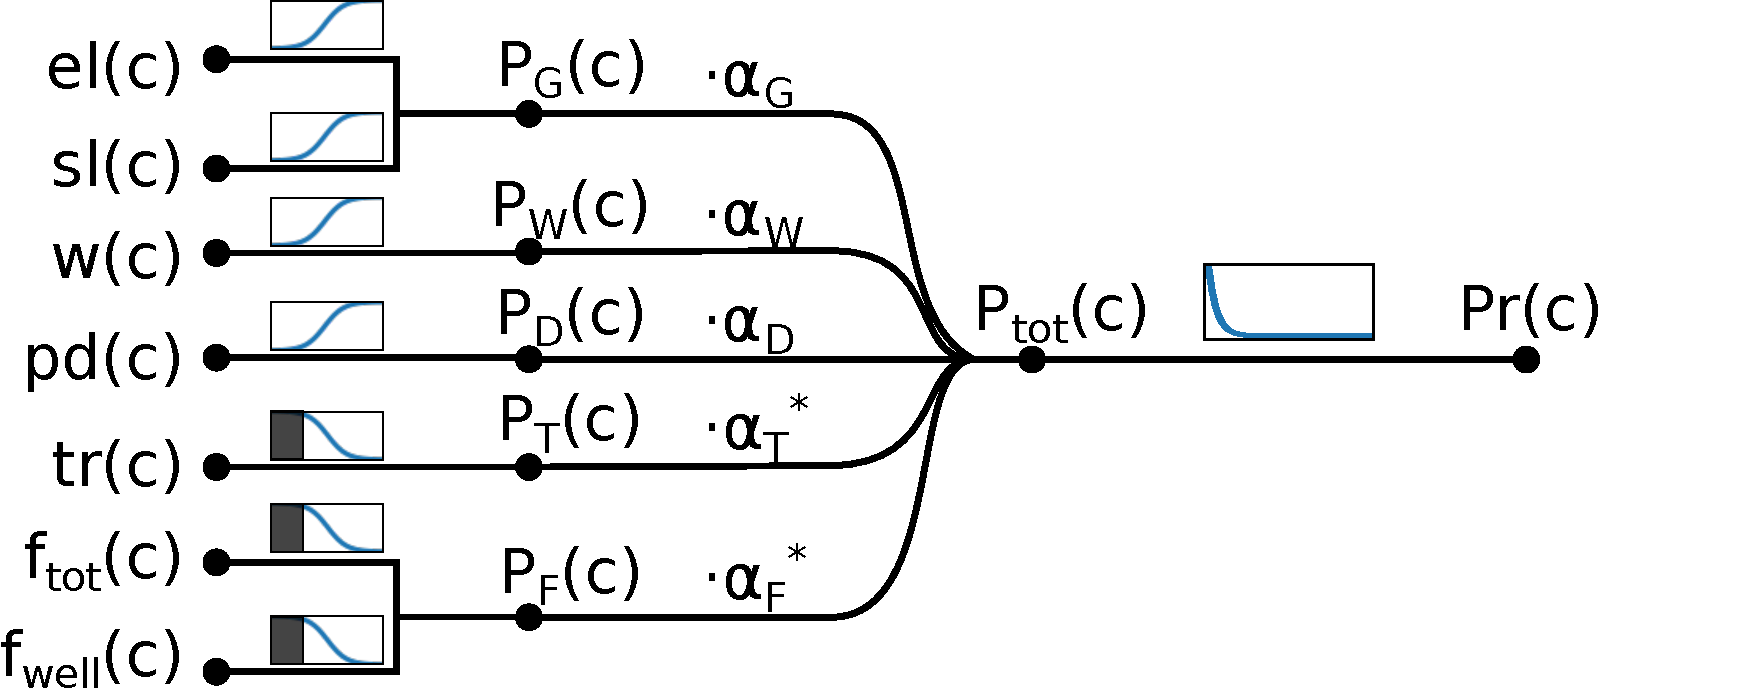
\includegraphics[width=1\textwidth]{images/SketchABM2/sketchMoving}
	\caption{A sketch of the calculation of the probability for agent $i$ to relocate its settlement to cell $c$: The category penalties ($P_{\rm G}$ for geography, $P_{\rm W}$ for freshwater proximity, $P_{\rm D}$ for population density, $P_{\rm T}$ for tree availability, $P_{\rm F}$ for farming land availability) are calculated via one or two characteristic evaluation variables described in the main text assuming a logistic functional dependence (red curves). 
	If two evaluation criteria are considered for one category, the resulting sub-penalties are averaged (crossings for $P_{\rm G}$ and $P_{\rm F}$).
	For $P_{\rm T}$ and $P_{\rm F}$, cells that do not have the minimum required resource availability are excluded (grey boxes).
	The total penalty for cell $c$, $P_{\rm total, \ i}(c)$ is then a linear superposition of all category penalties (with the weights $\alpha_{\rm T}^*$ and $\alpha_{\rm F}^*$ adjusted according to the tree preference $T_{\rm Pref, i}(t)$ in equation \ref{eq:vecalpha}).
	The final probability for a cell $c$ is derived as $Pr(c) \sim e^{-\gamma \cdot P_{\rm tot, \ i}(c)}$ (red line in the right part), with scaling factor $\gamma$.} 
	\label{fig:sketchmoving}
\end{figure}



% TOPIC: When does it occur, calc penalty in each day, \ldots
%With this procedure, agent's move (as resource availability becomes scarce or a subgroup splits from a large household) according to environmental features. 
%The specific settings create spatial patterns of settlement behaviour which in turn non-linearly change the agent-environment interaction and, thus, environment dynamics overall.

\paragraph{Computation Time of the Moving Process.}
The decision making process when an agent moves is the bottleneck w.r.t.\ computation time in the ABM.
A single evaluation process scales quartic with the grid resolution $\delta_{\rm x,y}$, i.e.\ $\mathcal{O}(\delta_{\rm x,y}^4)$: The overall number of cells to consider, $N_{\rm c}$, increases quadratic with $\delta_{\rm x,y}$ and the evaluation of penalties (e.g.\ summing up trees from cells in $C_{\rm T}(\tilde{c})$) for evaluation of a single cell also scales quadratic with the grid resolution.
In order to increase efficiency, I use dot products and distance matrix computation from the python packages \textit{numpy}\footnote{\citet{numpy}} and \textit{scipy}\footnote{\citet{scipy}}, both implemented in \CC.
Alternatively, one could adjust penalties (or characteristic variables) immediately when the agents interact with the environment, which would scale as $\mathcal{O}(\delta_{\rm x,y}^2\cdot N_{\rm agents}(t)\cdot N_{\rm timesteps})$ and, thus, likely obtain a faster implementation.
	
		
% Measure Agric Productivity in acres of high quality sites
% Why Wood is a primary resource
% Tree Pref changes quickly
% Mention non-reneqabl etc. earlier.
% Burning not really sure??
% Define SItes(c) as int(area)
% mention arable very early and farmed land
		
















%\section{Analysis, Experiments and Sensitivity Runs}
%\paragraph{Categorisation of Parameters}
%The resulting model has a multitude of parameters, settings and parametrisations often associated with large uncertainties. 
%There are in principle two different kinds of parameter choices described in the following paragraphs and summarised in Table \ref{tab:sensitivity}.

%\begin{adjustbox}{angle=90,caption={Choices of parameters for the standard configuration run and sensitivity analysis.}, float=table,}

\begin{flushleft}

\begin{sidewaystable}
	%\resizebox{\textheight}{!}{%
	  \hspace*{-3.3cm}\caption{Choices of parameters for the standard configuration run and sensitivity analysis.} %The upper half (separated by double line) mainly determines the aggregated population dynamics, the lower half determines the microscopic behaviour and thus influences mainly the spatial patterns.
	  \small
	\hspace*{-3.3cm}\begin{tabular}{P|W|W|M|K|Q}
%		Parameter &  Std Run & Fix? & Sensitivity Analysis \\ \hline
%		$t_{\rm arrival}$ & $800\, {\rm A.D.}$ & fix & Mostly only important for timing \\
%		$\mathbf{pop}_{\rm arrival}$ & $40$ & fix & -"- (within reasonable estimates)\\ \hline
%		 $F_\text{ Req, pP}$ & $0.5\, {\rm \frac{acres}{person}}$ & 2 & two different environmental scenarios \citep{Puleston2017}\\
%		 $F_\text{PI, [well, eroded, poor]}$ & $[0.8,\ 0.5,\ 0.1]$ & fix & strong impact (especially poor vs.\ well), estimated from \citet{Louwagie2006} \\
%		 $T_\text{Req, pP}$ & $5\, {\rm \frac{Trees}{person\cdot yr}}$ & 2 & strong impact 
%		 estimate from \citet{Brandt2015}, tested 

		\textbf{Parameter} & \textbf{Value} & \textbf{Unit} & \textbf{Reference} & \textbf{Description} & \textbf{Sensitivity Test}\\ \hline \hline
		$t_{\rm arrival}$ & $800$ &${\rm A.D.}$& \citet{Bahn2017} & Start of simulation & --\\
		$\mathbf{pop}_{\rm arrival}$ & $40$ & ${\rm ppl}$ & \citet{Brander1998} & Population at $t_{\rm arrival}$ & --\\ \hline
		 $F_\text{ Req, pP}$ & $0.5$ & ${\rm \frac{farming\ sites}{person}}$ & \citet{Puleston2017} & Required (optimal) farming sites per person (high N fix.) & $1.7$ (low N fix.) \\
		 $F_\text{PI, well}$ & $0.8$ & -- & \citet{Louwagie2006} & Productivity index of well-suited cell & -- \\
		 $F_\text{PI, eroded}$ & $0.5$ & -- & -- & Productivity index of eroded, well-suited cell & --\\
		 $F_\text{PI, poor}$ & $0.1$ & -- & \citet{Louwagie2006} & Productivity index of poorly suited cell & -- \\ 
		 $T_\text{Req, pP}$ & $5$ & $ {\rm \frac{Trees}{person \cdot yr}}$ & \citet{Brandt2015} & Required trees per person per year & $10$  \\
		  $T_\text{Pref, min}$ & $0.2$ & --&-- & Minimum tree preference of an Agent&  -- \\ 
		  $T_\text{Pref, max}$ & $0.8$ & --&-- & Maximum tree preference of an Agent&  -- \\
		  $T_\text{Pref, min}|_{\rm fisher}$ & $0.5$ & --&-- & Minimum Tree preference of a fisher agent&  -- \\
		  $N_\text{Fisher, Max}$ & $10$ & --&-- & Maximum number of fisher agents &  -- \\ \hline
		   $r_{\rm F}$ & $1$ & ${\rm km}$ & -- & Searching radius for farming site &  %$0.5$ (`smaller') and $2$ (`larger')\\
		  $0.5$ and $2$\\
		  $r_{\rm T}$ & $2$ & ${\rm km}$ & -- & Searching radius for trees &  %$1$ (`smaller') and $4$ (`larger')  \\ \hline 
		  $1$ and $4$\\ \hline 
		  $f_{\rm Tree\  Pref}$ & linear & -- & --&  Adaptation strategy to local tree decrease & delayed, faster, logistic \\ \hline
		  	$\mathbf{T}(t_\text{arrival})$ & $16\cdot10^6$ & Trees & \citet{Mieth2015} & Total number of trees before arrival  &  -- \\  
		  Tree Pattern & -- & -- & \citet{Bahn2017} & Uniform density for $el(c)<450{\rm m}$, $sl(c)<10^\circ$ & -- \\ \hline
		  $g_{\rm T}$ & $0$ & $\%/{\rm yr}$ & \citet{Hunt2007}; \ldots %\citet{Bahn2017} 
		  & Max (logistic) growth rate of trees ($0\hat{=}$`without') & `with'$^{\rm a}$ \\ \hline
		  Droughts& -- & -- & \citet{Rull2020} & Drying of Rano Raraku $800-1200$, $1570-1720\, {\rm A.D.}$ & -- \\ \hline 
		  
		  $g$-scale & $0.1$ & -- & \citet{Lee2008} & Scale of Gamma CDF for growth rate $g(H_{\rm i}(t))$ & -- \\
		  $H_{\rm equ}$  & $0.688$& -- & \citet{Puleston2017} & 
		  Happiness at which $g(H_{\rm equ})=1$$^{\rm b}$& $0.84$\\
		  
		  $g(H_{\rm i}(t)=1)$ & $0.7$ & $\%/yr$ & \citet{Bahn2017} & Initial growth rate (with unlimited resources) & -- \\ \hline
		  $pop_{\rm min}$ & 6 & ${\rm ppl}$ & -- & Minimum population of a household & --\\
		  $pop_\text{split, mean (std)}$  & $42\ (3) $& ${\rm ppl}$ & -- & Gaussian splitting probability of a large household & --\\
		  %		  $$ & 3& -- & -- & -- & -- \\
		  $pop_{\rm split}$ & 12 & ${\rm ppl}$ & -- & Population size of a new agent after splitting & --\\ \hline
		  
		  $r_{\rm M}$ & $5$ & ${\rm km}$ & -- & Moving radius (if $\mathbf{pop}(t)>5000$) & -- \\
		  
		  $x_{\rm P0.01}$/$x_{\rm P0.99}$ & \ldots & \ldots & \ldots & see Table \ref{tab:x01x09} & -- \\
		  $\vec{\alpha}$ & $\alpha_x=0.2$ & -- & -- & Weights for penalty categories ($x$) in moving decision & $\alpha_{\rm T,F} = 0.5$ \\
		  $\gamma$ & $20$ & -- & -- & Scaling factor: Total penalty to moving probability&  $0$, $1000$\\
		\end{tabular}
  \label{tab:sensitivity}
  	\begin{itemize}
  		  \setlength\itemsep{-8pt}
  	{\scriptsize
  	\item[a] With tree regrowth: $g_{\rm T} = 5\%/yr$, and `pop up' on barren cells ($0.5\%$ of carrying cap after 10 years) as in equation \ref{eq:treeupdate}.
  	\item[b] $H_{\rm equ}$ determines the shape of the Gamma CDF for $g(H_{\rm i}(t))$: $H_{\rm equ}=0.688$ \ra $shape = 1.95$, and  $H_{\rm equ}=0.84$ \ra $shape = 3$.
  }
  \end{itemize}
%\end{sidewaystable}
\end{sidewaystable}
\end{flushleft}
%\begin{threeparttable}
%\centering
%\begin{tabular}{P|S|H|Q|M|P}
%	$\mathbf{T}(t_\text{arrival})$ & $16\cdot10^6$ & Trees & \citet{Mieth2015} & Total number of trees before arrival  &  -- \\  
%	Tree Pattern & -- & -- & \citet{Bahn2017} & Uniform density for $el(c)<450{\rm m}$, $sl(c)<10^\circ$ & -- \\ \hline
%	$g_{\rm T}$ & $0$ & $\%/{\rm yr}$ & \citet{Hunt2007}; \citet{Bahn2017} & Max (logistic) growth rate of trees ($0\hat{=}$`without') & `with'\tnote{a} \\ \hline
%	Droughts& $800-1200$ \& $1570-1720$ & ${\rm A.D.}$ & \citet{Rull2020} & Drying of Rano Raraku & -- \\ \hline 
%	
% $g(H_{\rm i}(t))$ (scale) & $0.1$ & -- & \citet{Lee2008} & Scale of Gamma CDF describing an agent's growth rate $g(H_{\rm i}(t))$ & -- \\
% $H_{\rm equ}$  & $0.688$& -- & \citet{Puleston2017} & 
% Happiness at which $g(H_{\rm equ})=1$\tnote{b}& $0.84$\\
%
% $g(H_{\rm i}(t)=1)$ & $0.7$ & $\%/yr$ & \citet{Bahn2017} & Initial growth rate (with unlimited resources) & -- \\ \hline
% 		  $pop_{\rm min}$ & 6 & ${\rm ppl}$ & -- & Minimum population of a household & --\\
% $pop_\text{split, mean}$ $(pop_\text{split, std})$ & $42\ (3) $& ${\rm ppl}$ & -- & Gaussian splitting probability of a large household & --\\
% %		  $$ & 3& -- & -- & -- & -- \\
% $pop_{\rm split}$ & 12 & ${\rm ppl}$ & -- & Population size of a new agent after splitting & --\\ \hline
% 
% $r_{\rm M}$ & $5$ & ${\rm km}$ & -- & Searching radius for a new location (if $\mathbf{pop}(t)>5000$) & -- \\
%
%$x_{\rm P0.01}$/$x_{\rm P0.99}$ & \ldots & \ldots & \ldots & see Table \ref{tab:x01x09} & -- \\
% $\vec{\alpha}$ & $\alpha_x=0.2 \ \forall \ x$ & -- & -- & Weights for penalty categories in moving decision & $\alpha_{\rm T,F} = 0.5$ \\
% $\gamma$ & $20$ & -- & -- & Scaling factor for probability depending on the total penalty &  $0$, $1000$\\
%\end{tabular}
%	\begin{tablenotes}
%	\item[a] With tree regrowth: $g_{\rm T} = 5\%/yr$, and `pop up' on barren cells ($0.5\%$ of carrying cap after 10 years).
%%	\item[b] Corresponds to shape of the Gamma CDF with value $1.95$.
%	\item[b] This determines the shape of the Gamma CDF describing the growth rate of the human population, $g(H_{\rm i}(t))$: For $H_{\rm equ}=0.688$, $shape = 1.95$, for  $H_{\rm equ}=0.84$, $shape = 3$
%%	\item[d] Corresponds to shape of the Gamma CDF with value $3$.
%\end{tablenotes}
%\end{threeparttable}

%\paragraph{Parameters Mainly Influencing the Aggregate Population Size}
%The first category of parameters influences directly the island wide, aggregate population dynamics and peak population because they determine the amount of resource acquisition and availability per agent and the population growth with respect to harvest success (or agent's happiness): 
%\begin{itemize}
%	\item the resource requirements calculated from the constant farming requirement per person $F_\text{ Req, pP}$ in combination with the farming productivity indices $F_\text{PI, [well, eroded, poor]}$, the tree harvest requirement per person $T_\text{Req, pP}$ as well as the values for $T_\text{Pref, min}$, and with a lower importance $T_\text{Pref, max}$, $T_\text{Pref, min}|_{\rm fisher}$ and $N_\text{Fisher, Max}$
%	\item the initial number of trees $\mathbf{T}(t_\text{arrival})$ and (if regeneration is enabled) the tree regeneration parameters, i.e.\ the logistic growth rate $g_{\rm T}$, and pop up properties on barren land 
%	\item the demography model parameters, i.e.\ the shape and scale of the population size growth rate function depending on the harvest success $g(H_{\rm i}(t))$ and the initial population growth rate $g(H_{\rm i}(t)=1)$.
%\end{itemize}
%%These parameters have a direct influence on the dynamics of the aggregated population size and its peak value.
%Furthermore, the parameters $t_{\rm arrival}$ and $\mathbf{pop}_{\rm arrival}$ simply influence the timing of the dynamics.
%The uncertainties associated with these parameters are the main source for the  
%discrepancies between contradictory theories about the history of Easter Island.
%This model presented here does not aim to dispute one theory or the other.
%In fact, the model can re-create the proposed population dynamics by adjusting some of the parameters above.
%Hence, while choosing a standard set of parameters, I also investigate some alternative settings of these parameters (shown in Table \ref{tab:sensitivity}) giving rise to different proposed theories of pre-history population dynamics on Easter Island.
%
%\paragraph{Parameters Mainly Influencing the Spatial Patterns}
%The novel part of this study, however is the spatially explicit component and the stochastic, microscopic acting and decision making of the agents in the model.
%The values of parameters associated with this second category are even less known, but as described in the Introduction, reasonable assumptions on the values and functional dependences of the parameters can be made more naturally on the microscopic than the macroscopic level. The parameters in this category are related to the
%\begin{itemize}
%	\item household size, i.e.\ the maximum and minimum population size  of an agent ($pop_{\rm min}$, $pop_\text{split, mean}$, $pop_\text{split, std}$, $pop_\text{split}$)
%	\item resource search radii ($r_{\rm F}$, $r_{\rm T}$ (in combination with the initial spatial distribution of trees, i.e.\ $T(c,t=t_{\rm arrival})$ for cells $c$)
%	\item shape of the response of the tree preference to the changing local environment
%	\item decision making process when moving, i.e.\ the restricted moving radius $r_{\rm M}$, penalty categories and their logistic dependency specified by the thresholds $x_{\rm P0.01}$ and $x_{\rm P0.99}$, the weights $\vec{\alpha}$, and the scale parameter $\gamma$.
%\end{itemize}
%
%% Every Run is a realisation: 
%\paragraph{Analysis}
%Throughout the thesis, I have defined parameter setting for a standard run (details in Table \ref{tab:sensitivity}).
%I perform several sensitivity simulations (also described in Table \ref{tab:sensitivity}) and analyse the corresponding changes to this standard run in both categories of parameters related to the aggregate population dynamics and to the spatial patterns.
%Since multiple processes in the model are stochastic, each run is only a single realisation. 
%While the aggregated results do not differ much between runs with the same setting, the spatial pattern of deforestation varies in general. 
%I perform several ensemble runs, but there is no obvious way to obtain an aggregate spatial mean dynamics per se.
%Instead, variation in spatial patterns for the same experiment are described qualitatively in most cases and by defining distinct spatial regions and looking at their population dynamics separately. 
%
%% Standard Run with table and then Average and Std
%\paragraph{Standard Run and Experiments}

% Perform sensitivity analysis of second for different settings of first categories.

% From standard run, try different moving probabilities.

